\pdfoutput=1 % only if pdf/png/jpg images are used
%\documentclass[cits]{JINST}
\documentclass[a4paper,10pt]{article}
%\documentclass[a4paper,10pt]{scrartcl}
\usepackage{geometry}
\geometry{a4paper,left=34mm,right=34mm, top=24mm, bottom=32mm}
%\geometry{a4paper}
\raggedbottom
\widowpenalty=10000
\clubpenalty=10000 
\usepackage{graphics}  
\usepackage{graphicx}
\usepackage{subfigure}
\usepackage{amsmath}
\usepackage[amssymb]{SIunits}
%\usepackage[load-configurations=abbreviations,tight-spacing=true,separate-uncertainty,bracket-numbers = false]{siunitx} % JINST cannnot handle siunitx !!
\usepackage{nicefrac}
\usepackage[english]{babel}
\usepackage{lineno}
\usepackage{epstopdf}
\usepackage{stfloats}
%\usepackage{upgreek}
\usepackage{verbatim}
\usepackage{url}
\usepackage{xcolor}
%\usepackage{draftwatermark}
%\SetWatermarkScale{5}
%\usepackage{setspace}
%\doublespacing

%general stuff 
\newcommand{\e}{\ensuremath{\mathnormal{e}}}
\newcommand{\h}{\ensuremath{\mathnormal{h}}}
\newcommand{\eV}{\ensuremath{\mathnormal{eV}}}
\newcommand{\cspeed}{\ensuremath{\mathnormal{c}}}

%tscope specific
\newcommand{\DESY}{\ensuremath{\textrm{DESY}}}
\newcommand{\Datura}{\ensuremath{\textrm{DATURA}}}
\newcommand{\Duranta}{\ensuremath{\textrm{DURANTA}}}
\newcommand{\Mimosa}{\ensuremath{\textrm{MIMOSA\,26}}}
\newcommand{\noise}{\ensuremath{\xi_{\textrm{n}}}}
\newcommand{\epsdut}{\ensuremath{\mathnormal{\varepsilon_{\textrm{DUT}}}}}
\newcommand{\epsmimo}{\ensuremath{\mathnormal{\varepsilon_{\textrm{M26}}}}}
\newcommand{\dz}{\ensuremath{\textrm{d}z}}
\newcommand{\dzdut}{\ensuremath{\textrm{d}z_{\textrm{DUT}}}}

%resolutions
\newcommand{\sigmap}{\ensuremath{\sigma_{\textrm{pointing}}}}
\newcommand{\sigmatu}{\ensuremath{\sigma_{\textrm{t,u}}}}
\newcommand{\sigmatb}{\ensuremath{\sigma_{\textrm{t,b}}}}
\newcommand{\sigmat}{\ensuremath{\sigma_{\textrm{t}}}}
\newcommand{\sigmapGBL}{\ensuremath{\sigma_{\textrm{p,GBL}}}}
\newcommand{\sigmameas}{\ensuremath{\sigma_{\textrm{meas}}}}
\newcommand{\sigmadut}{\ensuremath{\sigma_{\textrm{DUT}}}}
\newcommand{\sigmai}{\ensuremath{\sigma_{\textrm{int}}}}
\newcommand{\sigmam}{\ensuremath{\sigma_{\textrm{M26}}}}
\newcommand{\sigmahat}{\ensuremath{\hat{\sigma}_{\textrm{int}}}}

%positions
\newcommand{\zdut}{\ensuremath{z_{\textrm{DUT}}}}
\newcommand{\zzz}{\ensuremath{z_{3}}}

%residuals
\newcommand{\rbiased}{\ensuremath{r_{\textrm{b}}}}
\newcommand{\runbiased}{\ensuremath{r_{\textrm{u}}}}
\newcommand{\rhat}{\ensuremath{\hat{r}_{\textrm{b}}}}
\newcommand{\pb}{\ensuremath{p_{\textrm{b}}}}


%software
\newcommand{\eudet}{\ensuremath{\textrm{EUDET}}}
\newcommand{\rawdataevent}{RawDataEvent }
\newcommand{\rawdataevents}{RawDataEvents }
\newcommand{\eudaq}{\ensuremath{\textrm{EUDAQ}}}
\newcommand{\EUTelescope}{\ensuremath{\textrm{EUTelescope}}}

%linenumbers
\setpagewiselinenumbers
\modulolinenumbers[5]

\makeatletter
\renewcommand{\maketitle}{\bgroup\setlength{\parindent}{0pt}
\begin{flushleft}
  \vspace*{10mm}
  \textbf{\huge\sffamily\@title}
  \vspace{5mm}
   
  \large \@author
\end{flushleft}\egroup
}
\def\@xfootnote[#1]{%
  \protected@xdef\@thefnmark{#1}%
  \@footnotemark\@footnotetext}
\makeatother

%\setlength\extrarowheight{5pt}
\renewcommand{\arraystretch}{1.25}
%\date{\vspace{-5ex}} %FIXME: remove for preprint


% \abstract{
% The status of the $\Datura$ Telescope at DESY is summarised and the performance is shown with two example studies. 
% The pointing resolution using a 6\,GeV $\e$-beam at the centre of the telescope is $\unit{5}{\upmu\meter}$.
% }

%\keywords{Pixel, CMOS, Beam telescope, resolution, tracker} % need to be specified during submission

\begin{document}
\linenumbers


%DESY 6
%D. Eckstein, 				doris.eckstein@desy.de
%T. Eichhorn, 				thomas.eichhorn@desy.de
%I. Gregor,				ingrid.gregor@desy.de
%C. Muhl,				carsten.muhl@desy.de
%H. Jansen, 				hendrik.jansen@desy.de
%R. Peschke,				Richard.Peschke@desy.de
%S. Spannagel,				simon.spannagel@desy.de

% Uni of Bristol 1
%D. G. Cussansm				David.Cussans@bristol.ac.uk

%DPNC 2
%E. Corrin,		SwiftKey	emlyn.corrin@gmail.com
%D. Hass, 		SRON: 		D.Haas@sron.nl

%IPHC Strasbourg, France 3
%Mark Winter				marc.winter@iphc.cnrs.fr
%Mathieu Goffe				mathieu.goffe@iphc.cnrs.fr
%Gilles Claus				gilles.claus@iphc.cnrs.fr 

%INFN Como 1
%Antonio Bulgheroni, 	KIT		antonio.bulgheroni@gmail.com

%Ex-DESY: 5
%H. Perrey, 				hanno@perrey.info
%Philipp Roloff,	CERN 		philipp.roloff@cern.ch
%I. Rubinskiy,		CFEl/CUIigor	igor.rubinskiy@cfel.de

\title{Performance of the EUDET-type\\ beam telescopes}
\author{
H.~Jansen${}^{\textrm{a,}}$\footnote[*]{Corresponding author: hendrik.jansen@desy.de},
S.~Spannagel${}^{\textrm{a}}$, 
A.~Bulgheroni${}^{\textrm{b,}}$\footnote{Now at KIT, Karlsruhe, Germany},
G.~Claus${}^{\textrm{c}}$,
E.~Corrin${}^{\textrm{d,}}$\footnote{Now at SwiftKey, London, UK},
D.~G.~Cussans${}^{\textrm{e}}$,
D.~Eckstein${}^{\textrm{a}}$, 
T. Eichhorn${}^{\textrm{a}}$, 
M.~Goffe${}^{\textrm{c}}$,
I.~M.~Gregor${}^{\textrm{a}}$, 
D.~Haas${}^{\textrm{d,}}$\footnote{Now at SRON, Utrecht, Netherlands},
C.~Muhl${}^{\textrm{a}}$,
H.~Perrey${}^{\textrm{a,}}$\footnote{Now at Lund University, Sweden}, 
R.~Peschke${}^{\textrm{a}}$, 
P.~Roloff${}^{\textrm{a,}}$\footnote{Now at CERN, Geneva, Switzerland}, 
I.~Rubinskiy${}^{\textrm{a,}}$\footnote{Now at CFEL, Hamburg, Germany}, 
M. Winter${}^{\textrm{c}}$\\
\vspace{3mm}
${}^{\textrm{a}}$ Deutsches Elektronen-Synchrotron DESY, Hamburg, Germany\\
${}^{\textrm{b}}$ INFN Como, Italy\\
${}^{\textrm{c}}$ IPHC, Strasbourg, France\\
%${}^{\textrm{c}}$ D\'epartement de physique nucl\'eaire et corpusculaire, University of Geneva, Switzerland\\
${}^{\textrm{d}}$ DPNC, University of Geneva, Switzerland\\
${}^{\textrm{e}}$ University of Bristol, UK
}
\maketitle


%-------------------
% \title{The EUDET-type Beam Telescopes}
% \author{
% H.~Jansen${}^{\textrm{a,}}$\thanks{Corresponding author: hendrik.jansen@desy.de}\,\,, 
% A.~Bulgheroni${}^{\textrm{b,}}$\thanks{Now at KIT, Karlsruhe, Germany},
% G.~Claus${}^{\textrm{c}}$,
% E.~Corrin${}^{\textrm{d,}}$\thanks{Now at Swiftkey, London, UK}\,\,,
% D.~G.~Cussans${}^{\textrm{e}}$,
% D.~Eckstein${}^{\textrm{a}}$, T. Eichhorn${}^{\textrm{a}}$, M. Goffe${}^{\textrm{c}}$,
% I.~M.~Gregor${}^{\textrm{a}}$, 
% D.~Haas${}^{\textrm{d,}}$\thanks{Now at SRON, Utrecht, Netherlands}\,\,,
% %  A. Kravchenko${}^{\textrm{a,}}$\thanks{Now at }\,\,, 
% H.~Perrey${}^{\textrm{a,}}$\thanks{Now at ESS, Lund, Sweden}\,\,, 
% R.~Peschke${}^{\textrm{a}}$, 
% P.~Roloff${}^{\textrm{a,}}$\thanks{Now at CERN, Geneva Switzerland}\,\,, 
% I.~Rubinskiy${}^{\textrm{a,}}$\thanks{Now at CFEl, Hamburg, Germany}\,\,\,\,, 
% S.~Spannagel${}^{\textrm{a}}$, 
% M. Winter${}^{\textrm{c}}$\\
% \vspace{3mm}
% ${}^{\textrm{a}}$ Deutsches Elektronen-Synchrotron DESY, Hamburg, Germany\\
% ${}^{\textrm{b}}$ INFN Como, Italy\\
% ${}^{\textrm{c}}$ IPHC, Strasbourg, France\\
% %${}^{\textrm{c}}$ D\'epartement de physique nucl\'eaire et corpusculaire, University of Geneva, Switzerland\\
% ${}^{\textrm{d}}$ DPNC, University of Geneva, Switzerland\\
% ${}^{\textrm{e}}$ University of Bristol, UK
% }
% \maketitle
%----------------

\begin{abstract}
\noindent
Test beam measurements at the test beam facilities of DESY have been conducted to characterise the performance of the EUDET-type beam telescopes originally developed within the $\eudet$ project. 
The beam telescopes are equipped with six sensor planes using $\Mimosa$ monolithic active pixel devices. 
A programmable Trigger Logic Unit provides trigger logic and time stamp information on particle passage. 
Both data acquisition framework and offline reconstruction software packages are available. 
User devices are easily integrable into the data acquisition framework via predefined interfaces.
 
The biased residual distribution is studied as a function of the beam energy, plane spacing and sensor threshold. 
Its width at the two centre pixel planes using all six planes for tracking in a 5\,GeV electron/positron-beam is measured to be $(2.88\,\pm\,0.08)\,\upmu\meter$.
Iterative track fits using the formalism of General Broken Lines are performed to estimate the intrinsic resolution of the individual pixel planes. 
The mean intrinsic resolution over the six sensors used is found to be $(3.24\,\pm\,0.09)\,\upmu\meter$.
With a 6\,GeV electron/positron beam, the track resolution halfway between the two inner pixel planes using an equidistant plane spacing of 20\,mm is estimated to $(1.78\,\pm\,0.03)\,\upmu\meter$
 assuming the measured intrinsic resolution. 
Towards lower beam energies the track resolution deteriorates due to increasing multiple scattering. 
Threshold studies show an optimal working point of the $\Mimosa$ sensors at a sensor threshold of between five and six times their RMS noise. 
Measurements at different plane spacings are used to calibrate the amount of multiple scattering in the material and allow for corrections to the predicted angular scattering for electrons beams. 
\end{abstract}


\tableofcontents
%\newpage


\section{Introduction}
\label{sec:intro}

%History of DESY beam telescopes, from Eudet to the present

Beam telescopes are a vital tools for sensor R\&D projects. 
These range from collider-specific detectors with high radiation-hardness requirements\,\cite{Nurnberg:2014aya, Garcia-Argos:2015zda},
 high resolution and low mass requirements\,\cite{HuGuo2010480}, and medical applications\,\cite{Ballabriga2011S15} to HV-CMOS studies\,\cite{1748-0221-7-08-C08002}, to name just a few.
Complementary to sensor simulations using finite element analysis tools, test beams studies are used at various stages including the development of either the sensor or the readout chip,
 and subsequently when testing a complete demonstrator with a full data acquisition system. 
%Also in future high-energy physics experiments pixel detectors will be used in the inner layers of the tracking devices. 
%The demands are challenging and range from high speed and high radiation-hardness for the high-luminosity LHC (HL-LHC)
% experiments\,\cite{Nurnberg:2014aya, Garcia-Argos:2015zda} to high resolution and low mass at the International Linear Collider (ILC)\,\cite{ILC} or at the Compact Linear Collider (CLIC)\,\cite{CLIC}. 
These studies are well suitable and often used for the evaluation of the performance of a detector prototype. % developed within the various R\&D projects. 
In order to facilitate these measurements a high-resolution pixel beam telescope was developed within the $\eudet$ project\,\cite{ref:eudetreport200902},
 with the clear guideline to allow for the integration of user data acquisition systems for a wide range of read-out schemes, latencies, and frequencies. 
Fast LHC-type devices need to be integrable in the same manner as slow calorimetric or rolling-shutter readout devices. 

Consisting of six pixel detector planes equipped with small-pitch $\Mimosa$ sensors,
 the mechanics for precise positioning of the device under test (DUT) and the telescope planes in the beam, trigger capabilities, and its data acquisition system, 
 the DESY-type beam telescopes meet the requirements in terms of easy integration capabilities, spatial resolution, and trigger rates. 
The telescope planes are designed and built to keep the material budget as low as possible in order to achieve an excellent pointing resolution
 even at the rather low DESY test beam energies of up to 6\,GeV.

Several replicas of the DESY-type beam telescope have been built:
 the AIDA telescope residing at the SPS, H6 (CERN), the ATLAS copy ACONITE, which will also be operated at H6, ANEMONE at ELSA (University of Bonn), the copy for the Carlton University called CALADIUM, 
 $\Datura$ at DESY and, currently under construction, $\Duranta$, which will also be operated at DESY. 
All replicas are build on the $\Mimosa$ sensors and use the same data acquisition system and framework. 
The results reported here are based on data taken with $\Datura$ at test beam area\,21 at {DESY-II} and with ACONITE at SLAC, ESTB and SPS, H6, but are applicable to all other copies. 

The paper is organised as follows: 
The beamlines relevant for the data analysed in this work are introduced in section~\ref{sec:beamlines}, followed by the description of the beam telescope
 and the data acquisition framework in sections~\ref{sec:tscope} and~\ref{sec:eudaq}, respectively.
Section~\ref{sec:offline} details the offline analysis and reconstruction software. 
Finally, in section~\ref{sec:trackres} results of the DESY-type beam telescope performance are presented. % and the pointing resolution for different telescope configurations at various beam momenta is shown. 
The measured data is complemented by analytic predictions using the concept of General Broken Lines (GBL)\,\cite{Kleinwort-2012}.
%With these GBL predictions at hand, the optimal telescope geometry can be calculated for a given set-up (DUT, cooling, ...) prior to the test beam.


\section{Beamlines}
\label{sec:beamlines}

For this work, data has been taken at three different test beam facilities, namely at {DESY-II}, at SPS~H6 and at SLAC~ESTB.
% Test beam in general and at DESY
%Test beam facilities have shown up as working horses for detector development for LHC upgrades as well as the future linear colliders.
The DESY-II electron/positron synchrotron at the DESY site in Hamburg has a circumference of 292.8\,m and is mainly used as an injector for the PETRA-III storage ring. 
However, it also supplies beam to three test beam areas, one  of them being the test beam area\,21.
%The circumference of the DESY-II ring is 292.8\,m. 
Its dipole magnets operate in a sinusoidal ramping mode with a frequency of 12.5\,Hz. 
Therefore, one DESY-II cycle takes 80\,ms, the bunch length is around 30\,ps. 
% Principle of Test beam generation 
The DESY-II synchrotron is equipped with movable carbon fibres. 
If these are positioned in the beam, bremsstrahlung photons are created leaving the beam line tangentially.
Subsequently, the photons are converted to electron/positron pairs on a secondary metal target. 
Their energy distribution reaches up to 6\,GeV. 
Using a dipole magnet, this secondary electron/positron beam is spread out.
A collimator can be used to select certain energy ranges of the beams reaching the experimental halls with an achievable rate of about $10$\,kHz to $100$\,kHz. 
%In optimal conditions, a maximal particle rate of $9$\,kHz at around 2.5\,GeV/$\cspeed$ can be reached. 
A more detailed description of the test beams at {DESY-II} is given in reference~\cite{EUDET-2007-11}.

% CERN and SLAC
%In addition to measurements at DESY\,II, the beam telescopes were also characterised at other test beam facilities: 
At CERN, the circular proton synchrotron SPS~\cite{SPS} of 6.9\,km length is the final injector of proton beams for the Large Hadron Collider. 
Additionally, it provides a proton beam on three secondary targets resulting in a mixed beam (electrons, hadrons, muons) with energies between 5\,GeV to 205\,GeV
 feeding up to seven beam lines in the SPS North Area, one of them being the H6 beam line. 
One beam spill contains up to $\sim 2\cdot10^8$\,particles and is 4.8\,s to 9.6\,s long. 
A spill occurs every 14\,s to 48\,s depending on the operation mode. 
% Talks when google: SPS CERN test beam
% 5 – 205 GeV/c
% Particle intensity max. 2*108 particles per spill
% spill length4.8 to 9.6 s 
% spill every 14s – ~48s
% more at: http://ps-schedule.web.cern.ch/ps-schedule/

At SLAC, the Linac Coherent Light Source incorporates a primary electron beam with up to 13.6\,GeV and a repetition rate of 120\,Hz~\cite{SLAC}.
Either this primary beam, or a secondary beam produced on a thin target can be sent to the End Station Test Beam (ESTB) with energies between 3.5\,GeV and 13.6\,GeV at 5\,Hz
 resulting in up to $10^{9}$ electrons per pulse.

%A beam pulse incorporates typically 109\,particles at 5\,Hz.\,\cite{d}
% https://portal.slac.stanford.edu/sites/ard_public/facet/newnav/Pages/tf/estb/ESTB-Beam.aspx

%Results on the resolution of the beam telescopes depending on different test beams and, thus, beam energies are described in section~\ref{sec:trackres}. 







\section{Components of the EUDET-type beam telescopes}
\label{sec:tscope}

The DESY-type beam telescope are tabletop tracking detectors featuring six pixelated silicon sensors, four scintillators with photo multiplier tubes (PMTs) for trigger purposes,
 a Trigger Logic Unit (TLU) providing trigger logic and time stamp information on particle passage, and a data acquisition system for the data readout. 
Figure\,\ref{fig:datura-tscope} shows the beam telescope with its sensor jigs, wherein the pixel sensors are embedded, with its auxiliary boards providing connections for power,
 sensor configuration, clock signals, and data transmission. 
The planes are organised in two telescope arms holding three sensors each. 
A DUT can be inserted between the arms or at either end of the beam telescope. 
In the Cartesian, right-handed coordinate system chosen, the $x$-direction points horizontally and $z$-direction along the beam.

\begin{figure}[tb]
	\center
	\includegraphics[width=.9\textwidth]{figures/DATURA.jpg}
	\caption[The $\Datura$ telescope]{The $\Datura$ beam telescope with its sensor planes on aluminium rails.
	The auxiliary boards with connections for clock signals, sensor configuration, and data lines are mounted at the top of the jigs.
	Coolant is provided to the jigs via the tubes.}
	\label{fig:datura-tscope}
\end{figure}
 
\subsection{Sensors and mechanics}
\label{sec:sensors}

The $\Mimosa$ detectors used for precise spacial measurement of particle trajectories are manufactured with the 350\,nm CMOS technology. 
Each $\Mimosa$ detector consists of pixels sized $\unit{18.4}{\upmu\meter} \times \unit{18.4}{\upmu\meter}$, which are arranged in 1152 columns and 576 rows.
This adds to a total of about four million readout channels covering an active area of about $\unit{10.6}{\milli\meter} \times \unit{21.1}{\milli\meter}$. 
The $\Mimosa$ sensors have been thinned down to $\unit{50}{\upmu\meter}$ and are protected on each side by $\unit{25}{\upmu\meter}$ lightproof Kapton foil. 
Free charge carriers produced in the underlying \unit{14}{\upmu\meter} epitaxial layer are mainly collected via diffusion. 
The binary resolution of $\unit{5.3}{\upmu\meter}$ can be improved by charge sharing, as will be shown in section~\ref{sec:trackres}.
%With the rising industrial interest in high resistivity epitaxial silicon for CMOS detectors the production cost of improved noise and radiation hardness parameters
% became already possible with ~400 Ohm·cm for 10 μm epitaxial layer for $\Mimosa$. 

The $\Mimosa$ sensors are read out with a rolling-shutter, taking 16\,cycles of an 80\,MHz clock per row, with all columns being read out in parallel. 
This allows for correlated double sampling and zero suppression on-chip with the digital circuitry placed outside the active pixel array. 
At this clock frequency, the $\Mimosa$ integration time equals $\unit{115.2}{\upmu\second}$ and allowing for about 8680 frames to be read out per second. 
The expected maximum rate of detectable particles through the active area estimates to be about $\unit{1}{\mega\hertz/\centi\meter^2}$ due to the limited on-chip buffer size. 
The detection threshold is programmable via so-called JTAG files. 
These provide configurations with different threshold levels in integer multiples $\noise$ of the RMS noise of the individual planes. 
A sensor threshold setting of six therefore corresponds to a collected charge in a single pixel of at least six times the noise. 
The average noise occupancy per read-out frame is measured to be smaller than $2\cdot10^{-5}$ at room temperature and a signal-to-noise threshold of six.

Every pixel sensor is mounted within an aluminium jig, three jigs are in turn mounted on each of the two aluminium arms. 
The jigs feature a beam window around the position of the sensor location, minimising the material budget. 
The overall material of the beam telescope thus amounts to $\unit{300}{\upmu\meter}$ of silicon and $\unit{300}{\upmu\meter}$ of Kapton. 
The two telescope arms, usually one up- and one downstream of the DUT, is movable along the direction of the beam in order to allow for variably sized DUTs to be fitted into the set-up. 
The minimal distance between two sensors is given by the jig thickness of 20\,mm, the maximal distance is restricted by the length of the aluminium arms to 150\,mm at equidistant spacing.
Furthermore, the jigs are cooled keeping the $\Mimosa$ sensors at a constant temperature allowing for stable operation.
The entire beam telescope is placed on a rotatable frame easing adjustment of its orientation parallel to the beam. 
Additionally, this frame is mounted on a sturdy structure providing stability over time and wheels for easy transportation. 

Important parameters are compiled in figure~\ref{fig:datura_sketch}. 
The distance between $\Mimosa$ planes is denoted as $\dz$, the distance between the DUT and its nearest neighbouring $\Mimosa$ planes $\dzdut$. 
The expression $\epsilon = \sum_i x_{i}/X_{0,i}$ defines the material budget of the scattering medium as the material thickness normalised to its radiation lengths,
 with values of $X_0 = 93.65\,\milli\meter$ for silicon, $X_0 = 3.042\cdot 10^{5}\,\milli\meter$ for dry air, and $X_0 = 285.6\,\milli\meter$ for Kapton, cf.~reference \cite{ref:x0values}.
The material budget of a $\Mimosa$ plane including a protecting Kapton foil on each side is $\epsmimo = 7.1\cdot10^{-4}$. 
Likewise, the DUT's material budget is called $\epsdut$ and includes the DUT itself and other material such as PCBs and cooling boxes.


\begin{figure}[tb]
	\center
	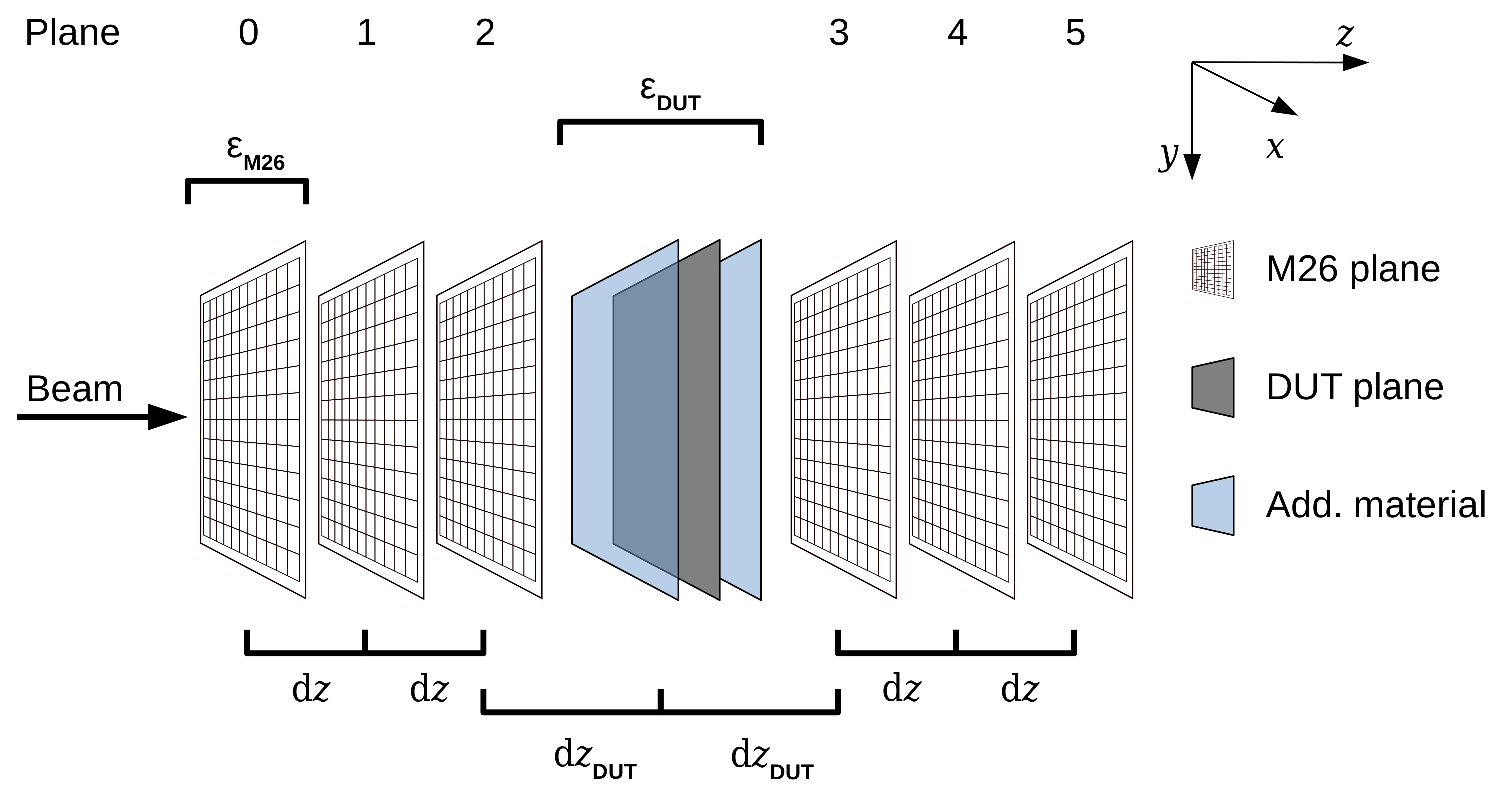
\includegraphics[width=.9\textwidth]{figures/sketch_tscope4}
	\caption[Sketch of the DESY-type telescope set-up]{Sketch of the DESY-type telescope set-up and its important parameters.}
	\label{fig:datura_sketch}
\end{figure}

\subsection{Trigger and DAQ system}

Four Hamamatsu PMT assemblies with scintillators and lightguides, two in front and two in the back of the telescope, define the spatial acceptance window for triggers. 
The crossed scintillators on either side of the beam telescope define a rectangular acceptance window of $10\,\milli\meter \times 20\,\milli\meter$ matching the $\Mimosa$ acceptance area. 
The TLU, based on a commercial Spartan\,3 board, features a coincidence unit with discriminator boards accepting up to four PMT inputs signals. 
Additionally, it is equipped with several custom-made add-on PCBs allowing for an easy integration of user DAQ systems. 
Providing a programmable logic, the TLU  takes a trigger decision and distributes the trigger signal to all DAQ systems.
As interface to the beam telescope DAQ and other DUTs, the TLU provides RJ45 connectors with four LVDS pairs carrying the trigger clock, the busy line, the reset line, and a trigger line. 
The data clock and the busy line are inputs to the TLU, whereas the reset and the trigger line are outputs. In addition, a LEMO interface is available providing trigger output and inputs for the busy and reset signals.

The TLU accepts a busy signal from each integrated device individually halting the issue of the next trigger if the busy signal is high. 
The handling of the trigger/busy signals can be done in three handshake modes, one being the ``no-handshake'' mode,
 in which the TLU issues a fixed-length pulse on the trigger line with the busy line being disregarded. 
In simple handshake mode, the assertion of a trigger is replied by the DUTs by asserting a signal on the busy line. 
The TLU then de-asserts the trigger, and waits for busy going low on the busy line in order to be able to issue a subsequent trigger.
The normal handshake uses the same scheme as in the simple trigger mode, but additionally trigger data is transferred on the trigger line:
After the trigger has been de-asserted, the trigger number is clocked out via this line using the rising edges of the trigger clock as clock enable for the shift register holding the trigger data. 
The reset line is used to signal the reset of the timestamp counter.

The $\Mimosa$ sensors provide zero-suppressed hit data over a flat ribbon cable to the auxiliary boards, which provide RJ45 connectors to connect them with the
 data concentrator board collecting the data from all six sensors and the trigger/busy lines from the TLU. 
A 52-pin cable then transports the data and the TLU trigger/busy lines in parallel into a FlexRIO board, which is equipped with analogue-to-digital converters and an FPGA. 
The $\Mimosa$ data from the rolling-shutter readout is written continuously to RAM without taking into account the trigger information. 
The data is then available via direct memory access to the DAQ software framework and an event is written to disk in normal handshake mode, only if a trigger has been raised for a certain telescope readout frame. 



\section{The EUDAQ data acquisition framework}
\label{sec:eudaq}

Pasting  from other another section:

EUDAQ serves as a tool set and an integration layer for the user DAQ system(s), providing the communication protocols for them to participate in a common DAQ. 

EUDAQ is a modular cross platform data Acquisition System designed in the context of the \eudet test beam Telescopes. 
It consist of completely independent modules such as run-control, log-Collector, Data-Collector and Producer. 
The communication between individual modules is done via TCP/IP therefore it is possible to run each module on a separate PC. 


\begin{figure}[tb]
	\center
	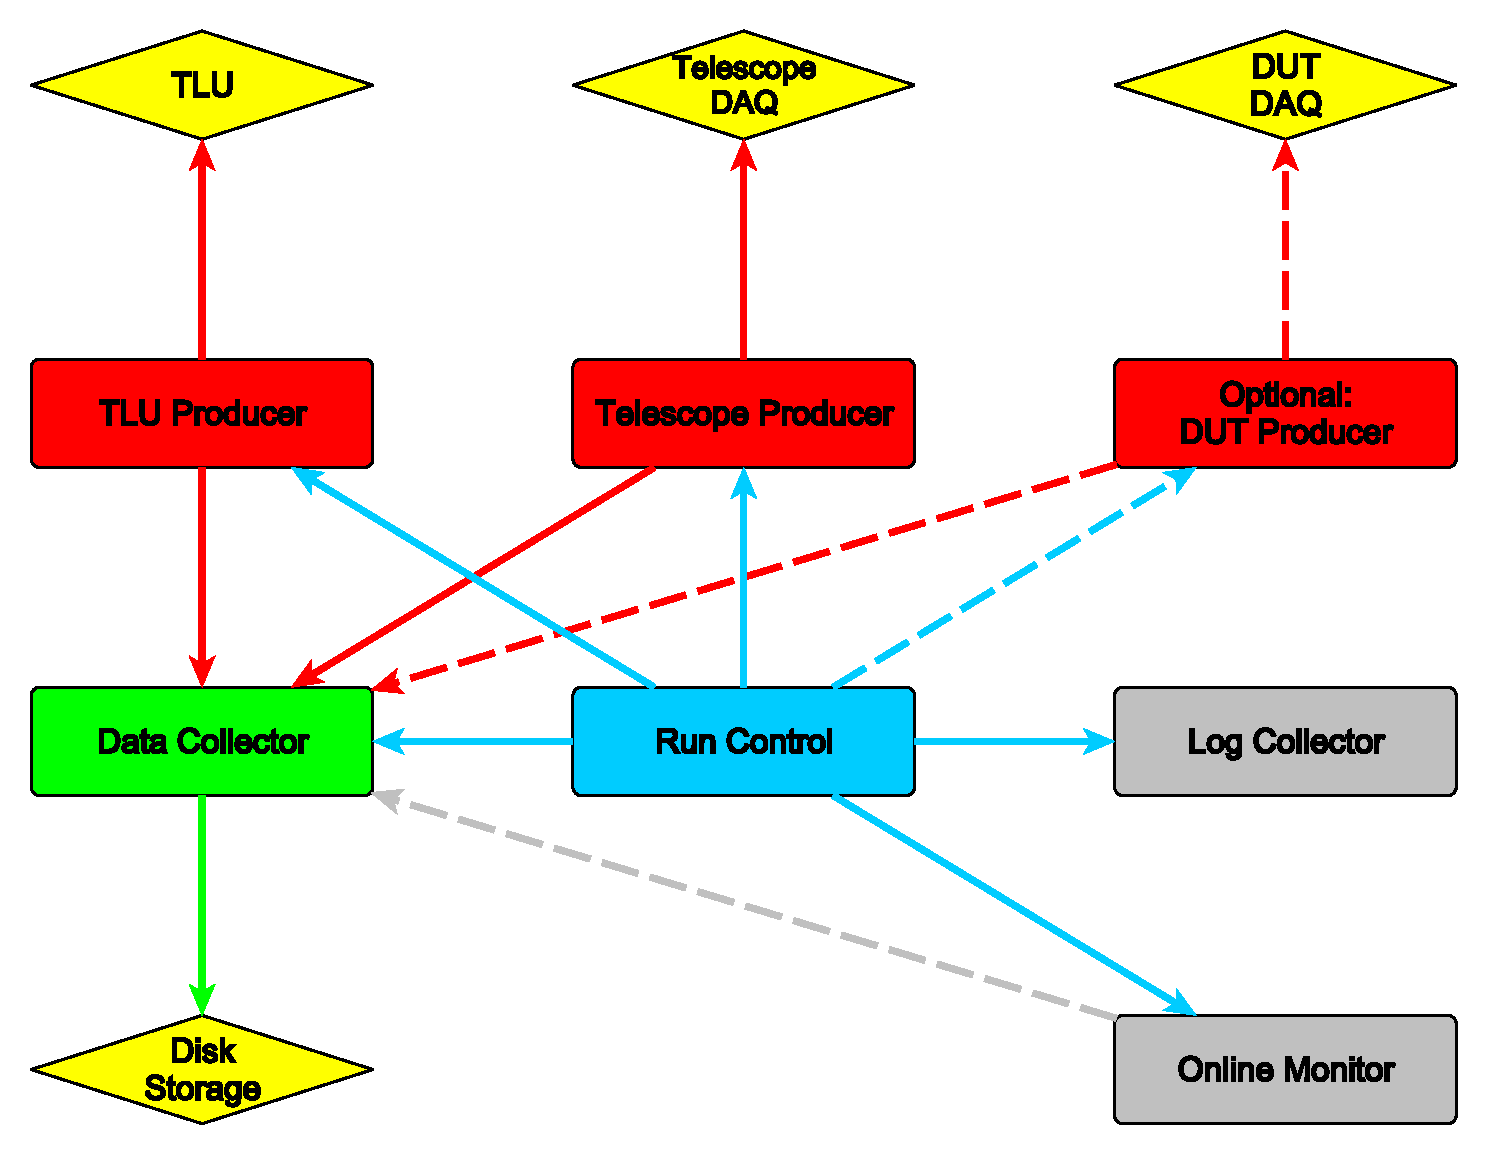
\includegraphics[width=.55\textwidth]{figures/eudaq}
	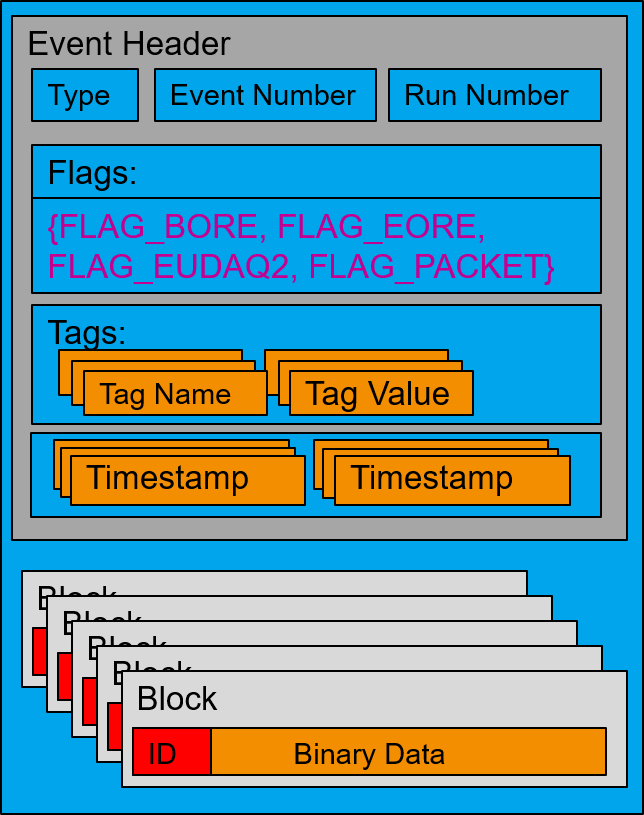
\includegraphics[width=.38\textwidth]{figures/rawdataevent.png}
	\caption[DAQ_System]{(A) Hardware and software layout of the DAQ system. (B) \rawdataevent}
	\label{fig:todo}
\end{figure}

% \begin{figure}[tb]
% 	\center
% 	
% 	\caption[DAQ_System]{\rawdataevent}
% 	\label{fig:todo}
% \end{figure}



The Run-Control is the central point for human interactions. 
From it the producer are configured, started, stopped and terminated. 
Currently there are two implementation of the Run-Control one command line version called TestRunControl and one GUI version Called euRun. 
Both have the about same functionality. 
The LogCollector receives all status/error messages that are produced by any of the producer. 
It has the possibility to filter for different warning levels. 
The DataCollector has a direct connection do all the producer. 
\eudaq 1.x is an event based DAQ system, therefore the Data-Collector expects that all producer send one event per trigger that they have reserved from the TLU. 
And that all events from different producer share a common trigger number by which they get merged into one container event called Detector-Event. 
The Data-collector has the possibility to do some basic sanity checks on the events like event number mismatch. 
The Producer handles the communication between the \eudaq framework and the user DAQ system. 
The user has to write its own Producer class which inherits from the abstract class producer. 
This class encapsulates the TCP/IP communication. 
The user needs to implement four virtual functions which handle the transit from one state to another. 
The producer has three states: unconfigured, configured and running. 
The configuration file is a plain text file which contains a section for each producer. 
Each sections contains tag-value pairs for the configuration of the producer. 
Sections for producer that are currently not connected are ignored. 
The basic event type that is used for user's data is the \rawdataevent. 
\rawdataevents are separated by the sub event type. 
A string which identifies the producer it belongs to. 
The sub event type is used to determine the corresponding data converter plugin. 
The \rawdataevent has the possibility to store tag value pairs as well as plain binary data. 
The ConverterPlugins are used to convert the data from plain binary data to pixels hits. 
The ConverterPlugin is explicitly not called from the DataCollector this makes it possible that the data collector can handle unknown data types. 
The \eudaq Framework comes with an online monitor which can either run online during the data taking or offline on files on disk. 
It produces hit-map and correlation-plots for all known producer types. 


\section{Offline analysis and reconstruction using EUTelescope}
\label{sec:offline}


The EUTelescope package \cite{ref:eutelwebsite} provides software tools for offline analysis and reconstruction of telescope test beam data. 
EUTelescope is embedded into the ILCSoft framework~\cite{ref:eudetmemo_2009_12} which provides the basic building blocks for offline analysis such as a data model (Linear Collider I/O, \emph{LCIO}),
a geometry description language (\emph{GEAR}) and the central event processor (\emph{Marlin}).

% thomas: this should be a reference to ilcsoft, not: \cite{EUDET-2008-48}.

EUTelescope comes with its own job submission framework \emph{jobsub} that allows to run analysis jobs locally or to submit them to larger computing clusters such as NAF.

Marlin allows the modular composition of analysis chains for various applications since every task is implemented as an independent \emph{processor} that is called by Marlin. 
The processors expose a set of parameters to the user which can be configured and loaded at runtime via so-called \emph{steering files} in XML format.
This way the Marlin/Processor architecture gives a lot of flexibility to the end user. 

EUTelescope provides several processors for Marlin implementing algorithms necessary for a full track reconstruction and data analysis of beam test experiments. 
Figure~\ref{fig:offline:strategy} shows the analysis strategy of the framework starting from the recorded detector response to the final aligned particle tracks. 
%An overview of the processor range provided by EUTelescope is given in \cite{EUDET-2007-20}.
For low-energy beams such as the DESY-II test beam facility multiple scattering is the dominating source of track resolution uncertainties (cf.\,Sec.~\ref{sec:multiplescattering})
Therefore EUTelescope provides advanced algorithms such as General Broken Lines (GBL) \cite{Kleinwort-2012} for tracking which accounts for scattering in all material present in the beam. 
In addition, precise software alignment can be performed using the Millipede-II algorithm \cite{Blobel-2006}.

\begin{figure}[tbp]
\center
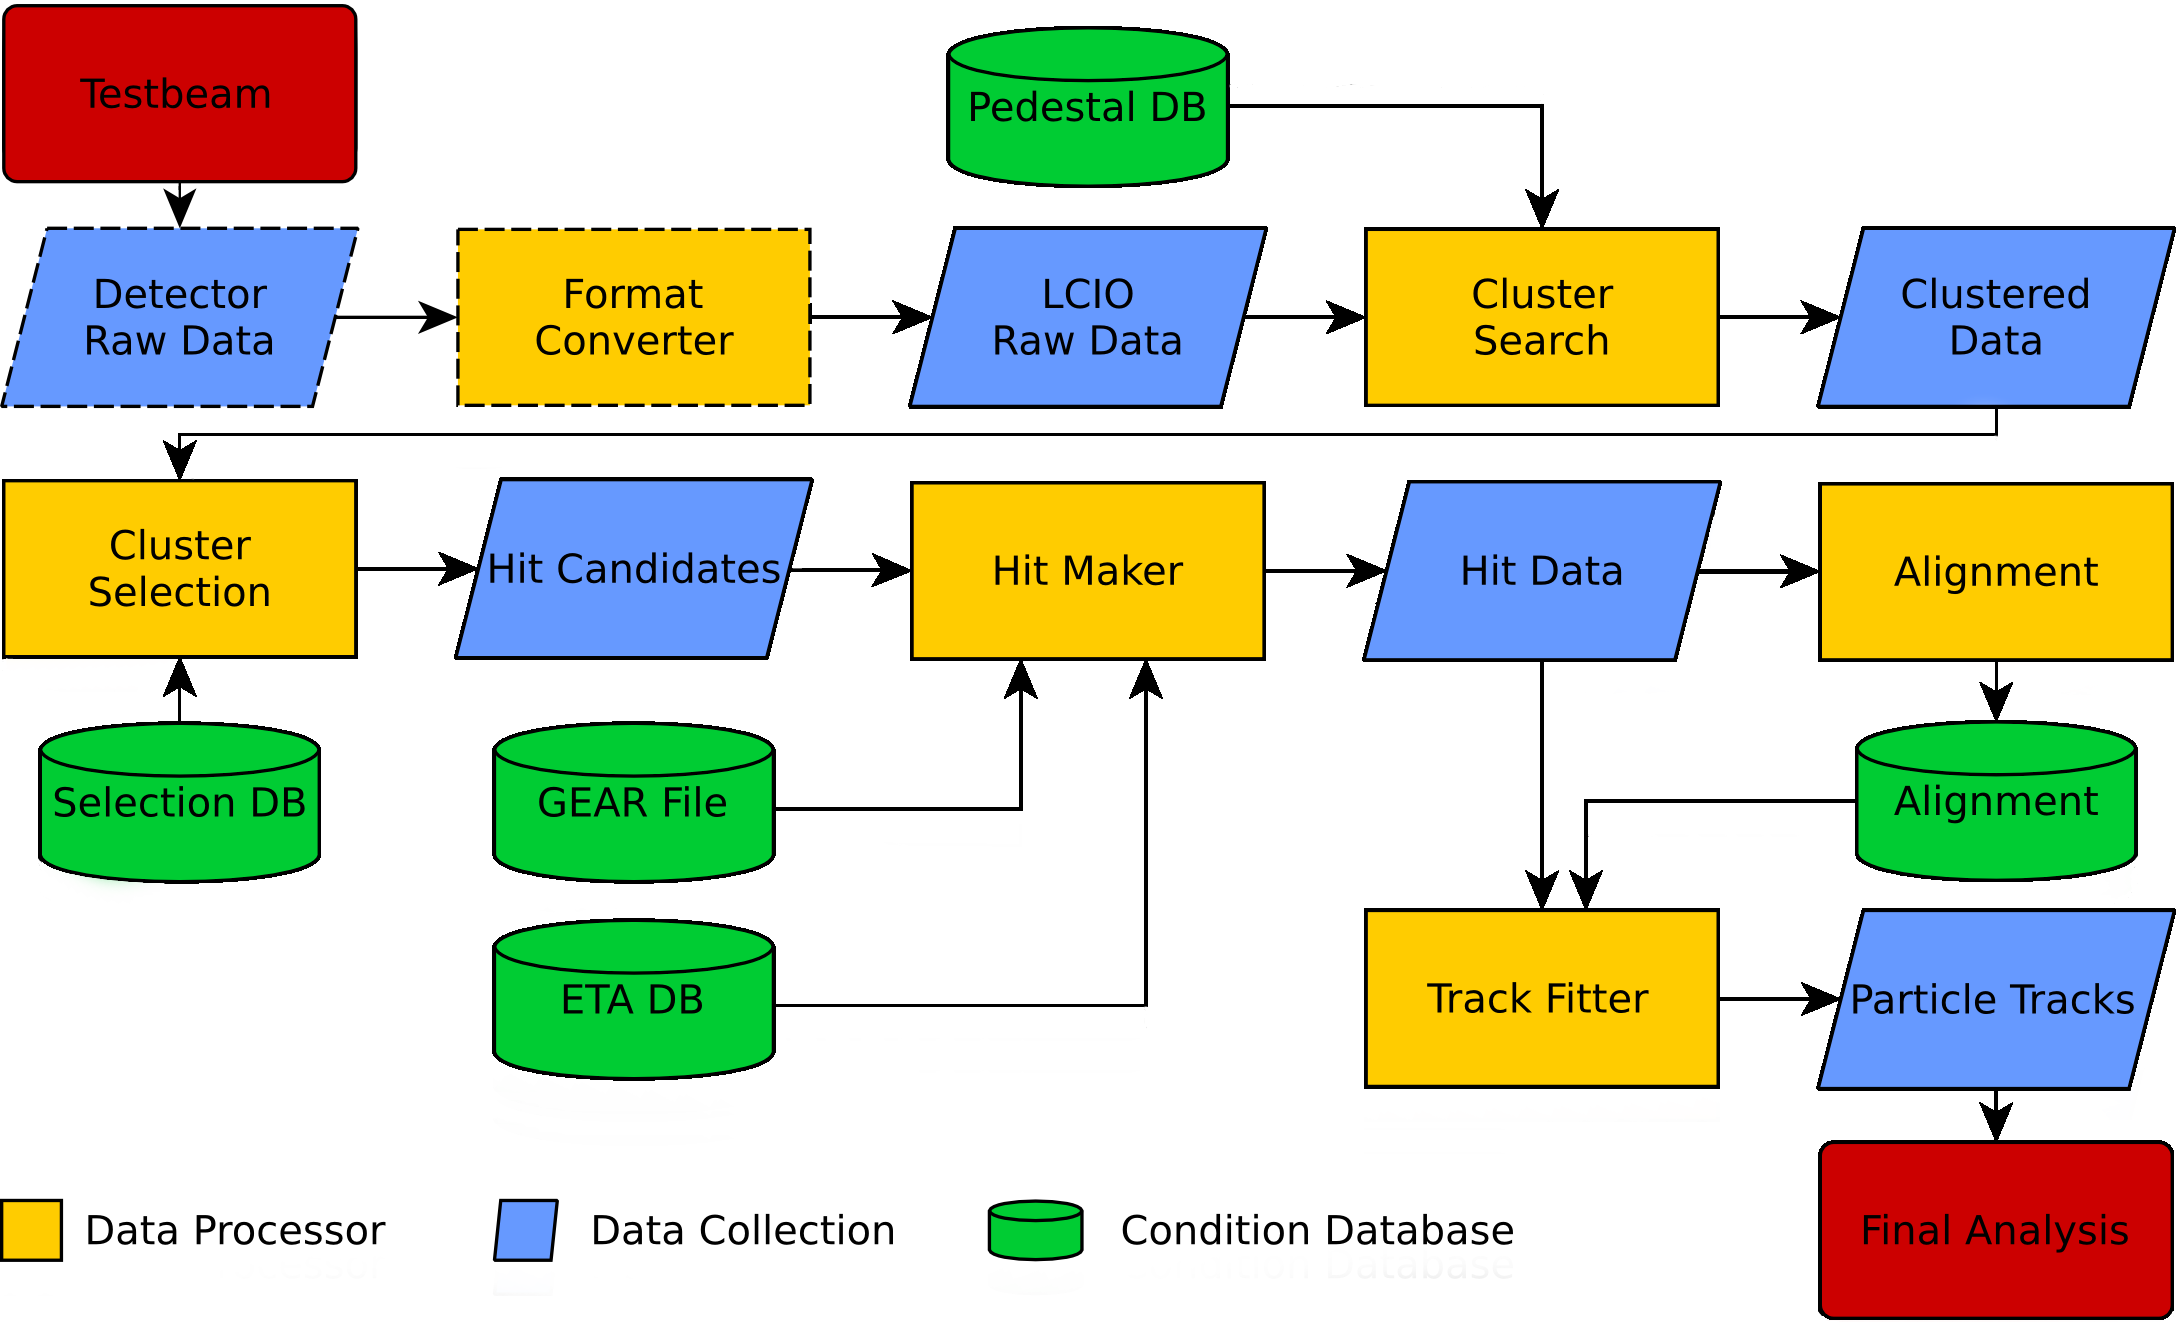
\includegraphics[width=.9\textwidth]{figures/eutel-strategy.png}
\caption[The EUTelescope data analysis strategy]{Schematic of the overall telescope data reconstruction and analysis strategy of the EUTelescope framework.
EUTelescope provides processors for all steps except for the ones with dashed outline; these have to be implemented by the user.}
\label{fig:offline:strategy}
\end{figure}




\section{Track resolution studies}
\label{sec:trackres}

The data presented were taken in $2015$ using $\Datura$, a $\eudet$-type beam telescopes, which was operated with EUDAQ, cf.~section~3 and~4. 
The results presented in this section have been obtained using the EUTelescope software described in section~\ref{sec:offline}.
The set-up does not include any additional DUT, only six $\Mimosa$ telescope planes. 
Track fits are performed using the GBL formalism and track residuals, i.e.\ the distance between the track fit and the measured hit,
 are calculated for each telescope plane. 
 

\subsection{Data analysis flow}
\label{sec:datura-nodut}

After conversion from raw $\Mimosa$ data, a hot pixel search is performed marking pixels with firing frequencies above a certain threshold.
Clusters are formed from fired, adjacent pixels and translated from two-dimensional entities on the individual telescope planes into hits in a global three-dimensional reference frame.
Those clusters containing at least one hot pixel are removed from the analysis. 
Track triplets are built from hits in the three upstream and three downstream planes separately: 
A straight line from one hit in each outward plane (plane\,0 and 2, plane\,3 and 5) is combined with a matching hit in the centre plane of the upstream or downstream trio, i.e. plane\,1 or plane\,4. 
Triplet isolation is ensured by rejecting all triplets whose extrapolation features distances to other triplet extrapolations that fall below $\unit{300}{\upmu\meter}$ at a chosen $z$-coordinate.
The $z$-coordinate chosen is the centre between plane\,2 and plane\,3. 
Matching triplets are identified by isolated triplets that intersect at $\zdut$ within a square with edge length smaller than $\unit{100}{\upmu\meter}$. 
In turn, GBL tracks are formed by the six hits belonging to the matched triplets. 
For offline alignment the GBL tracks are passed to Millepede-II in order to determine shift and rotation alignment constants for every telescope plane.
After applying the alignment constants, the above track finding is repeated, and the final GBL tracks are calculated. 
These tracks can be formed in a \textrm{biased} or in an \textrm{unbiased} form, where biased tracks include the measured hit information of every plane in contrast to unbiased tracks,
 that omit the hit information of the plane under investigation. 
Additionally, the tracking efficiency for the $\Mimosa$ sensors is calculated. 

\subsection{Multiple scattering and residuals}
\label{sec:resmultiple}

The figure of merit for a beam telescope is its track resolution\footnote{also called pointing resolution} $\sigmatb$ ($\sigmatu$).
It defines the precision with which a particle trajectory can be determined for an biased (unbiased) track. 
This quantity is a function of the track path, i.e.\ it is not constant along the trajectory. 
%The timing resolution is largely dependent on the readout speed of the used sensors, their buffer sizes and the data acquisition system. 
It depends on the intrinsic resolution $\sigmai$ of the sensors, that have been used to measure the hits belonging to the track, the number of hit measurements and their positions
 as well as the multiple scattering of the beam particles.
Various methods exist to perform the calculation of the track resolution. 
In the formalism of GBL, the track resolution results from a single, global $\chi^2$-fit of a track model to all measured hits including their measurement uncertainties (intrinsic resolution)
 and scattering angle uncertainties along the trajectory. 
% 
%The resolution of a telescope $\sigma_{\textrm{Tel}}$ can be expressed by
%
%\begin{equation}
%\label{eq:telescopepointing}
%\sigma_{\textrm{Tel}}^2 = k \cdot \sigmai^2
%\end{equation}
%
%\noindent
% with the geometric scaling factor $k$ in turn written as
%
%\begin{equation}
% k = \frac{\sum_i^N z_i^2}{N \cdot \sum_i^N z_i^2 - \left( \sum_i^N z_i \right)^2} \,,
%\end{equation}
%
%\noindent
% assuming all $N$ telescope planes have the same intrinsic resolution $\sigmai$. 
%The distance of the $i$-th telescope plane to the DUT positioned at $z=0$ is then $z_i$ .
%For a symmetric set-up with the DUT at the centre of the telescope and the up- and downstream planes equally spaced, $k$ reduces to $k = 1/N$. 
%
Multiple Coulomb scattering is the term used to describe the deflection of a charged particle traversing any medium.
The angular scattering distribution is centred around $0$
 and the width depends on the particle energy, particle type and the radiation length of the matter traversed~\cite{ref:scatteringhighland}.
An approximation for high energy protons, that is accurate to 11\,\% for all atomic numbers $Z$, yields a closed form for the distribution width in the transverse plane~\cite{ref:PDG-2014}

\begin{equation}
\label{eq:multiplescattering}
\Theta_{0} = \frac{13.6\,\mega\electronvolt}{\beta c p} \cdot z
\sqrt{\varepsilon}
\cdot \left( 1 + 0.038 \ln{\left( \varepsilon \right) } \right) \,,
\end{equation}

\noindent with the velocity $\beta c$, the momentum $p$ and the charge number $z$ of the traversing particle. 
The expression $\epsilon = x \per X_0$ is the material budget, as defined in section~\ref{sec:sensors}.
%
Equation~(\ref{eq:multiplescattering}) shows the advantage of using thin sensors, since the angular deflection due to multiple scattering increases with material budget.
This is especially important at low-energy beams, such as the DESY-II test beam, as the distortion increases towards lower energies.
As the beam particles interact with the sensors and the air, contributions to the amount of multiple scattering from both have to be considered.
At high-energy hadron beams, the contribution from multiple scattering can in general be neglected. 
 
The biased (unbiased) residual defined as a quantity per track is the spacing between the measured hit and the biased (unbiased) track fit. 
With a known or estimated biased track resolution, i.e.\ all $\sigmai(z_i)$ are known or estimates exist,
 the width of the distribution of the biased residuals for a set of tracks can be expressed for all positions $z = z_i$ as

\begin{equation}
 \label{eq:telescoperesolutionequation1}
 \rbiased^2(z) = \sigmai^2(z) - \sigmatb^2(z).
\end{equation}

\noindent
If the hit measurement of a DUT at $\zdut$ or of a telescope plane at position $z_i$ is not included in the fit,
 the width of the distribution of the unbiased residuals at these positions reads~\cite{ref:eudetreport200902}
 
\begin{equation}
\runbiased^2(z) = \sigmai^2(z) + \sigmatu^2(z).
\label{eq:telescoperesolutionequation2} 
\end{equation}

\noindent
Both the biased and the unbiased residual distributions are a function of the track resolution and therefore have the same dependencies.
It should be noted that the unbiased track resolution at a sensor plane can be larger than the intrinsic resolution. 
On the contrary, the biased track resolution is always smaller than or equal to the intrinsic resolution at the sensor planes. 

The biased pull of a track is defined as the ratio of the biased residual over the predicted biased residual width

\begin{equation}
 \textrm{pull}_{\textrm{b}} \equiv \pb = \frac{\rbiased}{\sqrt{\sigmai^2 - \sigmatb^2}}.
 \label{eq:pull}
\end{equation}

\noindent
The biased pull distributions are normally distributed and centred at 0 with a width of 1, if the material and the scattering therein is known and correctly described. 
A width larger than one results from an underestimated residual prediction $\sqrt{\sigmai^2 - \sigmatb^2}$, which in turn stems from either an underestimated intrinsic resolution
 or an overestimated track resolution. 
The latter is caused by either an overestimated material budget or overestimated deflection angles. 


A critical aspect of this analysis is the choice between biased and unbiased residuals. 
In principal, both choices lead to compatible results if the material in the beam and the deflection due to multiple scattering therein is correctly described. 
%With biased residuals, only one fit has to be performed, whereas for unbiased residuals, a new fit has to be formed for every plane under investigation. 
The impact of systematic uncertainties on the result, however, is different, as more information is used in the biased track fits. 
The material thicknesses and the amount of multiple scattering therein are only known with a certain accuracy affecting the track resolution, and thereby also the predicted residual width, 
 and hence the derived intrinsic resolution. 
%Especially the Highland formula is only accurate to about 11\,\%. 
If the pulls distribution resembles $N(0,1)$, equations~(\ref{eq:telescoperesolutionequation1}) and~(\ref{eq:telescoperesolutionequation2}) hold and the systematic uncertainties of the intrinsic resolution
 are estimated by calculating the effect of uncertain beam energy and uncertain deflection angle using the GBL formalism. 
Firstly, the residuals have been obtained from data assuming an intrinsic resolution of $\sigmai = \unit{3.3}{\micro\meter}$ and secondly the track resolution is calculated. 
Finally, the intrinsic resolution is calculated as $\sigmai = \sqrt{\rbiased^2 + \sigmatb^2}$ or $\sigmai = \sqrt{\runbiased^2 - \sigmatu^2}$ for biased and unbiased track fits, respectively. 
The beam energy is varied by 5\,\% and the deflection angle by 10\,\%. 
All systematic uncertainty contributions for the two set-ups are listed in table~\ref{tab:uncerts} exemplary for plane\,0.
It shows, that the choice of biased track fits results in smaller systematic uncertainties compared to unbiased track fits. 
Additionally, there is a systematic uncertainty of the method itself, as it predicts slightly different intrinsic resolutions for each plane, which changes between geometries,
 i.e.\ it is not dominantly caused by an actual difference in intrinsic resolution. 
The spread in intrinsic resolution over all planes is 1\,\% and 2\,\% for the wide and the narrow geometry, respectively. 

\begin{table}[tbp]
 \begin{center}
  \begin{tabular}{r|r|c|c|c||c}
  $\sigma_{\sigmai}$ in \% & × & $E\pm5\,\%$ & $\Theta\pm10\,\%$ & fit range & $\sqrt{\sum x_i^2}$\\ \hline
  biased   &  20 mm & 0.3 & 1.1  & 0.3 & 1.2 \\
  ×        & 150 mm & 0.10 & 0.13 & 0.05 & 0.17\\
  unbiased &  20 mm &   3 & 6    & 4  & 8\\
  ×        & 150 mm & n/a & n/a  & n/a & \\
  %× & × & × & ×
  \end{tabular}
    \caption[Systematic uncertainties for plane\,0]{Systematic uncertainties in determination of the intrinsic resolution for plane\,0, are listed for biased and unbiased track fits and the two geometries.
  For unbiased tracks in the wide geometry, the uncertainty of the intrinsic resolution could not be calculated as the measured residual is smaller than the calculated track resolution.}
  \label{tab:uncerts}
 \end{center}
\end{table}

The rather large uncertainty of the Highland formula and hence significant impact on the final results can be diminished: 
In case the Highland formula underestimates the actual straggling of beam particles in the given material, the predicted track resolution is systematically affected, and therefore the pull distribution. 
Hence, the estimator $\sigmahat$ does not converge towards the true $\sigmai$, but towards a larger value and vice versa. 
Since the intrinsic resolution is independent of the plane spacing $\dz$, a comparison at two precisely measured spacings allows for a calibration of $\Theta_0$ at a given beam energy. 
To this end, a global energy dependent factor $\kappa$ is introduced that is constant as a function of sensor threshold and geometry

\begin{equation}
 \Theta_{\textrm{corr}} = \kappa(E) \cdot \Theta_0.
 \label{eq:thetacorr}
\end{equation}

\noindent
The value $\kappa$ is found when the average of the intrinsic resolution over the six planes for $\dz = 150\,\milli\meter$ matches the average of the intrinsic resolution for $\dz = 20\,\milli\meter$. 
The uncertainty of $\kappa$ is defined as the range for which the average intrinsic resolution of the wide configuration equals the central value plus/minus one standard deviation of the narrow one. 
If $\kappa$ differs significantly from one and/or depends on the beam energy is to be determined with data. 


\subsection{Performance measurements with DATURA}
\label{sec:measurements}

Measurements of particle trajectories were performed to verify the performance of the $\Datura$ telescope at various beam energies, sensor thresholds, and sensor spacings. %~\cite{ref:thomas}.
The biased residual and biased pull distributions have been obtained for every sensor plane as described in sections~\ref{sec:datura-nodut} and~\ref{sec:resmultiple}. 
% By considering one telescope plane as a DUT, equation~(\ref{eq:telescoperesolutionequation}) is modified under the assumption that $\sigmai = \sigma_{\textrm{DUT}} = \sigma_{\textrm{M26}}$,
%  leading to
% 
% \begin{equation}
% \label{eq:telescoperesolutionequation_2}
% \sigmameas^2 = \sigma_{\textrm{M26}}^2 \cdot \left( 1 + k_5 \right) +
% \sigma_{\textrm{MS}}^2\,,
% \end{equation}
Since the intrinsic resolution is not a priori known, an initial estimate of the intrinsic resolution $\sigmahat$ is used as an input to the GBL track fitting. 
The width of the pull distributions therefore differs from 1 and is iteratively used to update the estimate $\sigmahat$.
This procedure converges towards the true intrinsic resolution within the uncertainties and yields compatible results for the two different geometries for an appropriate choice of $\kappa$. 
It should be noted that the systematic uncertainty of the converged estimate is independent of the iteration process.
\footnote{I.e., an initial estimate close to the converged value does not yield smaller uncertainties on the converged value compared to a bad initial estimate.}
%A mismatch in intrinsic resolution for the two cases is corrected by varying $\kappa$, cf.~equation~(\ref{eq:thetacorr}) and repeating the iterative method until the intrinsic resolutions equal


\begin{figure}[tbp]
  \centering
  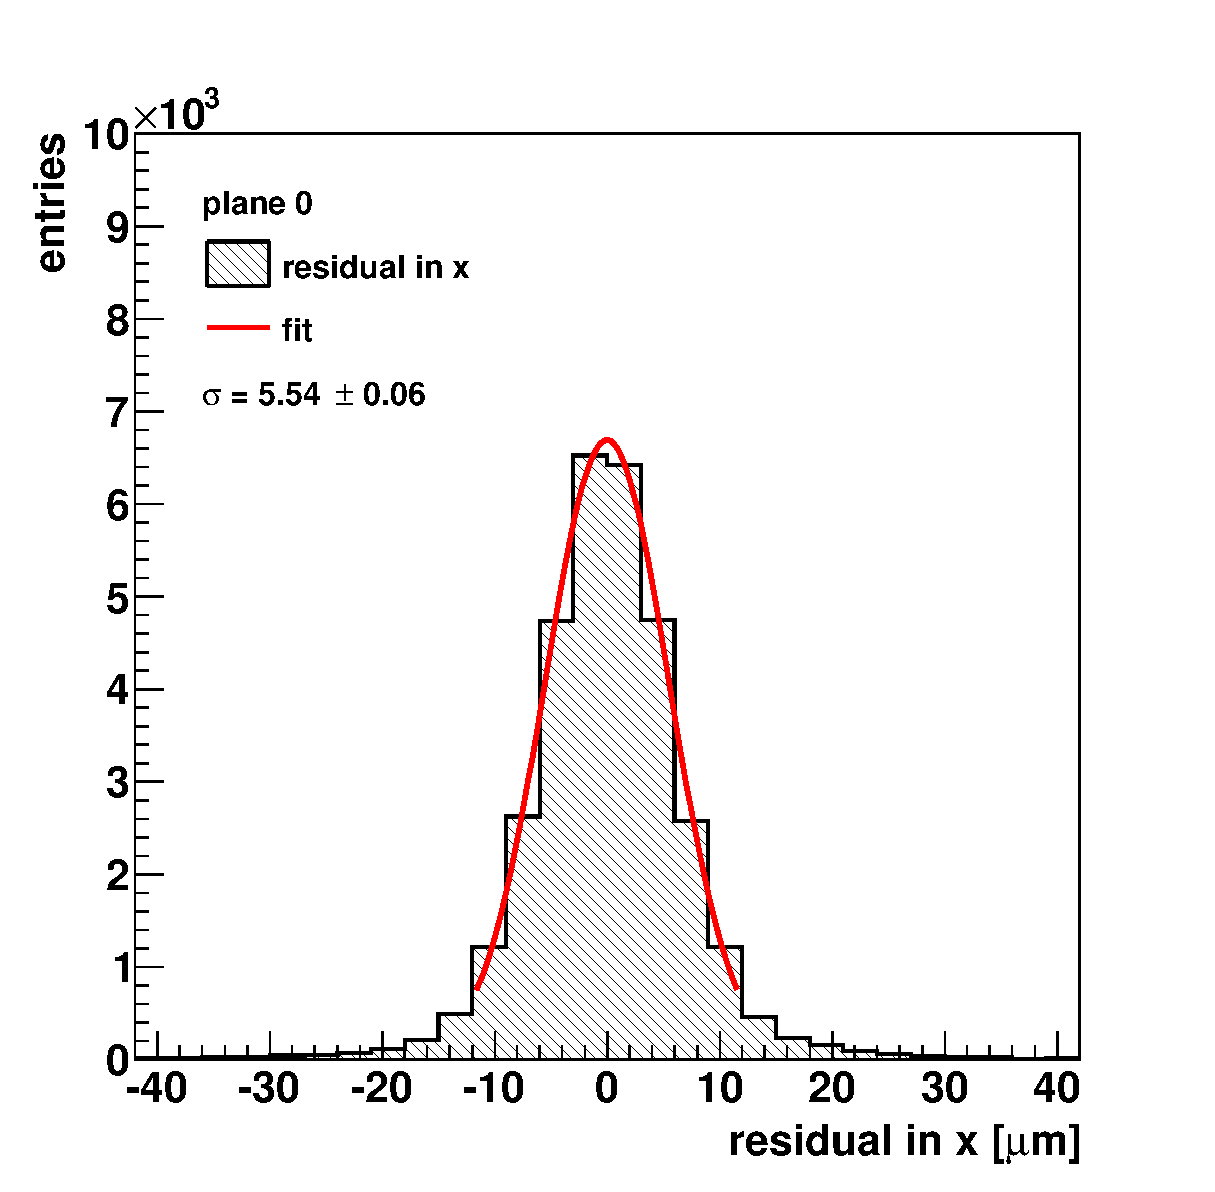
\includegraphics[width=0.49\textwidth]{figures/0x} \put(-50,155){(A)}
  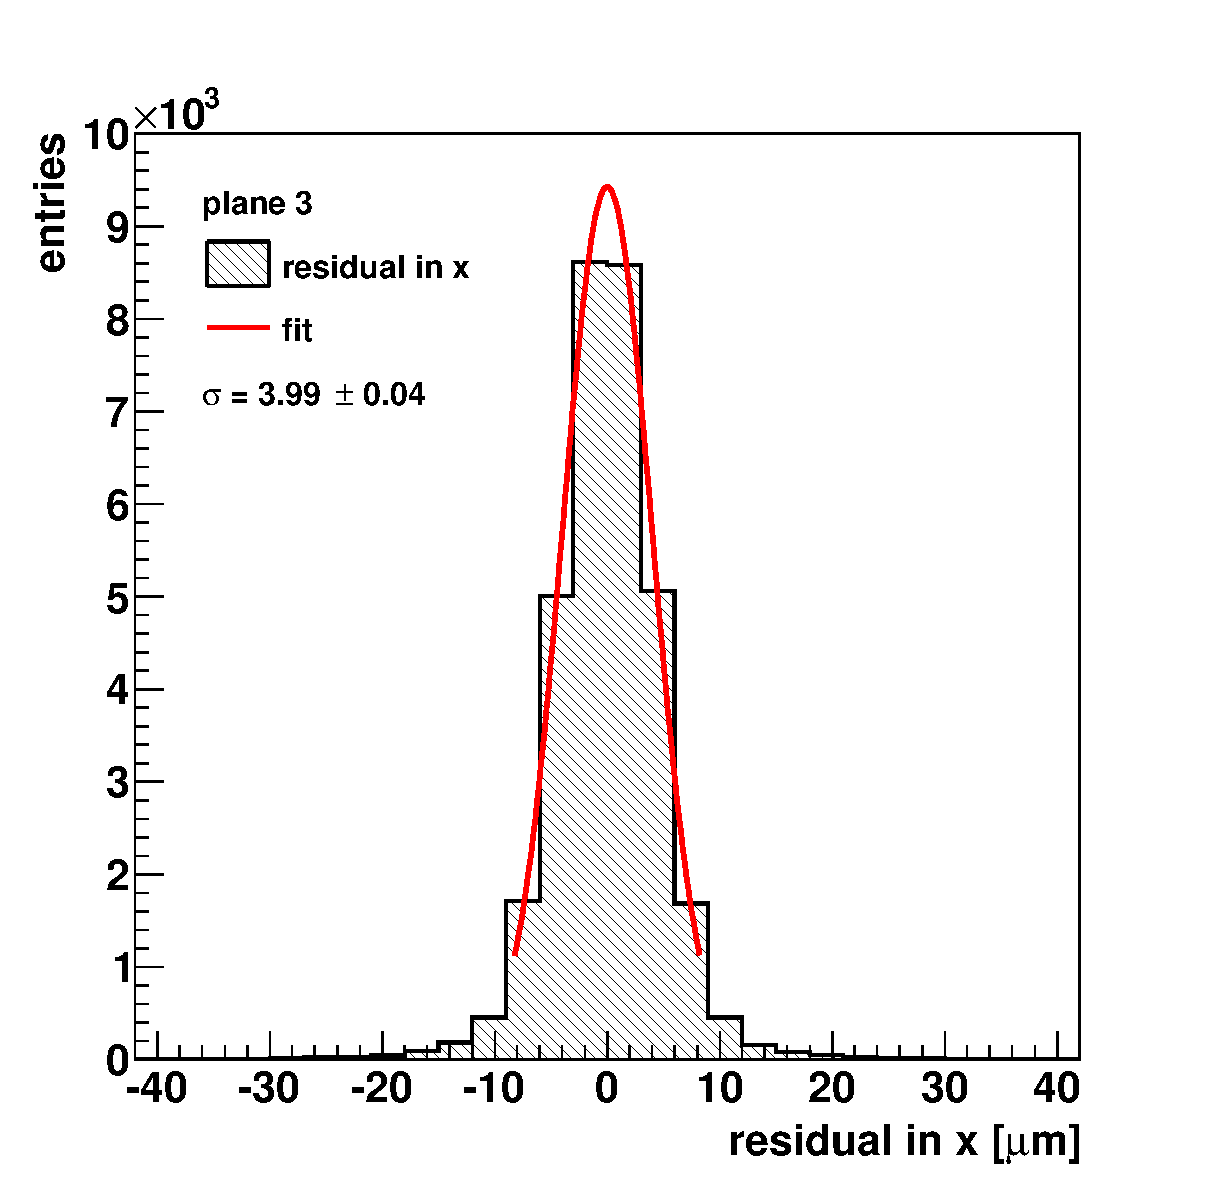
\includegraphics[width=0.49\textwidth]{figures/3x} \put(-50,155){(B)}\\
  %\includegraphics[width=0.45\textwidth]{figures/resis_upstream/1x.pdf}
  %\includegraphics[width=0.45\textwidth]{figures/resis_upstream/1y.pdf}
  %\includegraphics[width=0.45\textwidth]{figures/resis_upstream/2x.pdf}
  %\includegraphics[width=0.45\textwidth]{figures/resis_upstream/2y.pdf}
  %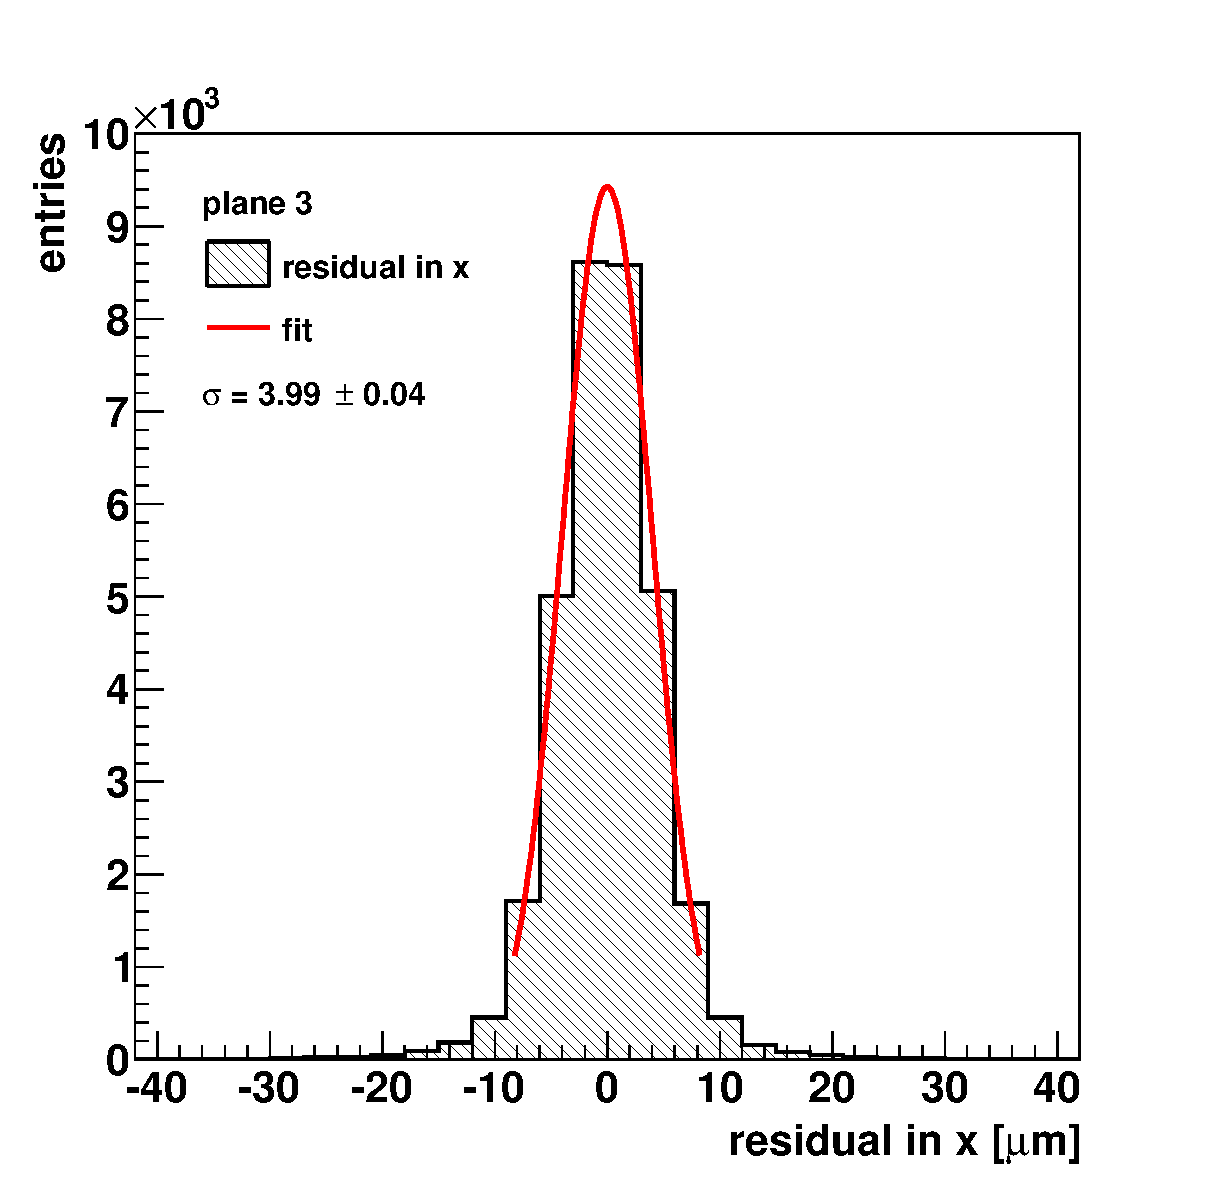
\includegraphics[width=0.49\textwidth]{figures/3x} \put(-50,155){(C)}
  %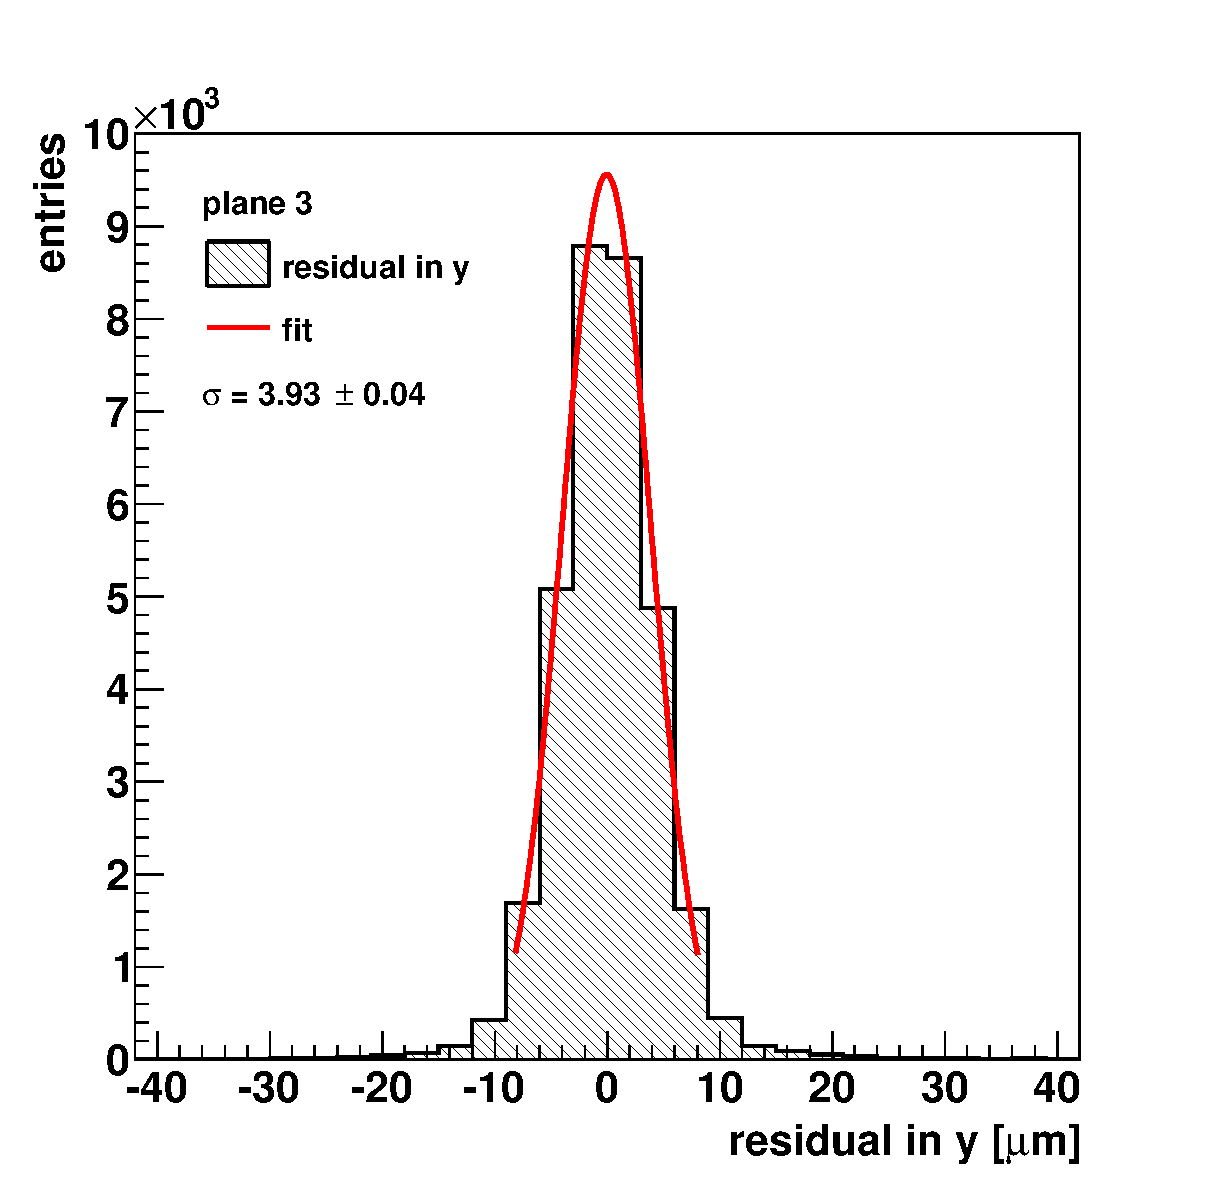
\includegraphics[width=0.49\textwidth]{figures/3y} \put(-50,155){(D)}
  %\includegraphics[width=0.45\textwidth]{figures/resis_downstream/4x.pdf}
  %\includegraphics[width=0.45\textwidth]{figures/resis_downstream/4y.pdf}
  %\includegraphics[width=0.45\textwidth]{figures/resis_downstream/5x.pdf}
  %\includegraphics[width=0.45\textwidth]{figures/resis_downstream/5y.pdf}
  \caption[Residual examples to determine the $\Datura$ telescope's resolution]{
  Biased residual distributions measured with the $\Datura$ telescope at 6\,GeV with a plane spacing of $\dz = 20\,\milli\meter$. 
  The measured residuals in the $x$-direction for plane $0$ (A) and plane $3$ (B) are shown.}
  \label{fig:residualexample1}
\end{figure}

\noindent
%with $k_5$ being the geometric scaling factor for a telescope consisting of five planes. 
%The value of $k_5$ depends on the geometry itself and on which telescope plane is considered as DUT. 
%This configuration with five planes used as beam telescope and one plane as DUT is referred to as \textit{gauge configuration}. 

Figure~\ref{fig:residualexample1} shows an example of converged biased residual distributions in $x$ for a telescope sensor spacing of $\dz = 20\,\milli\meter$,
 a beam energy of 6\,GeV, and a sensor threshold setting of $\noise = 6$. 
According results for the $y$-direction, further planes and the wide geometry are omitted. 
The distributions are fitted with a Gaussian, from which the residual width $\rbiased$ is determined. 
For plane\,3, the biased residual width in te $x$-direction is 

\begin{equation}
\left( 2.88\,\pm\, 0.01 \right)\,\micro\meter. 
\end{equation}

\noindent
It should be noted, that the residuals feature non-Gaussian tails, as is expected from the underlying physics of the scattering mechanism~\cite{ref:PDG-2014}. 
The measured resolution used in this work is defined as the width of a Gaussian fit on the centre $95.5\,\%$ (2.0 standard deviations) of the residual distribution.
The biased residual width for the outer plane\,0 is smaller than the width obtained from plane\,3.
This is expected due to the fact that the track extrapolation to the inner sensors is done from both sides, and hence is comparatively more precise than for the outer sensors,
 where the extrapolation can only be performed from one direction. 
Therefore, in equation~(\ref{eq:telescoperesolutionequation1}) the difference between $\sigmai$ and $\sigmatb$ decreases from the centre sensor planes to the outer ones. 

% \begin{figure}[hbtp]
% \centering
% 
% \caption[Residual examples to determine the DATURA telescope's
% resolution. Downstream lever arm]{Residual examples to determine the DATURA
% telescope's resolution from the downstream lever arm. From top to bottom: The
% measured residuals for planes $3$, $4$ and $5$, left for $X$ direction, right
% for $Y$ direction. Each sensor plane was considered as a passive layer during
% the track reconstruction.}
% \label{fig:residualexample2}
% \end{figure}

\begin{figure}[btp]
  \centering
  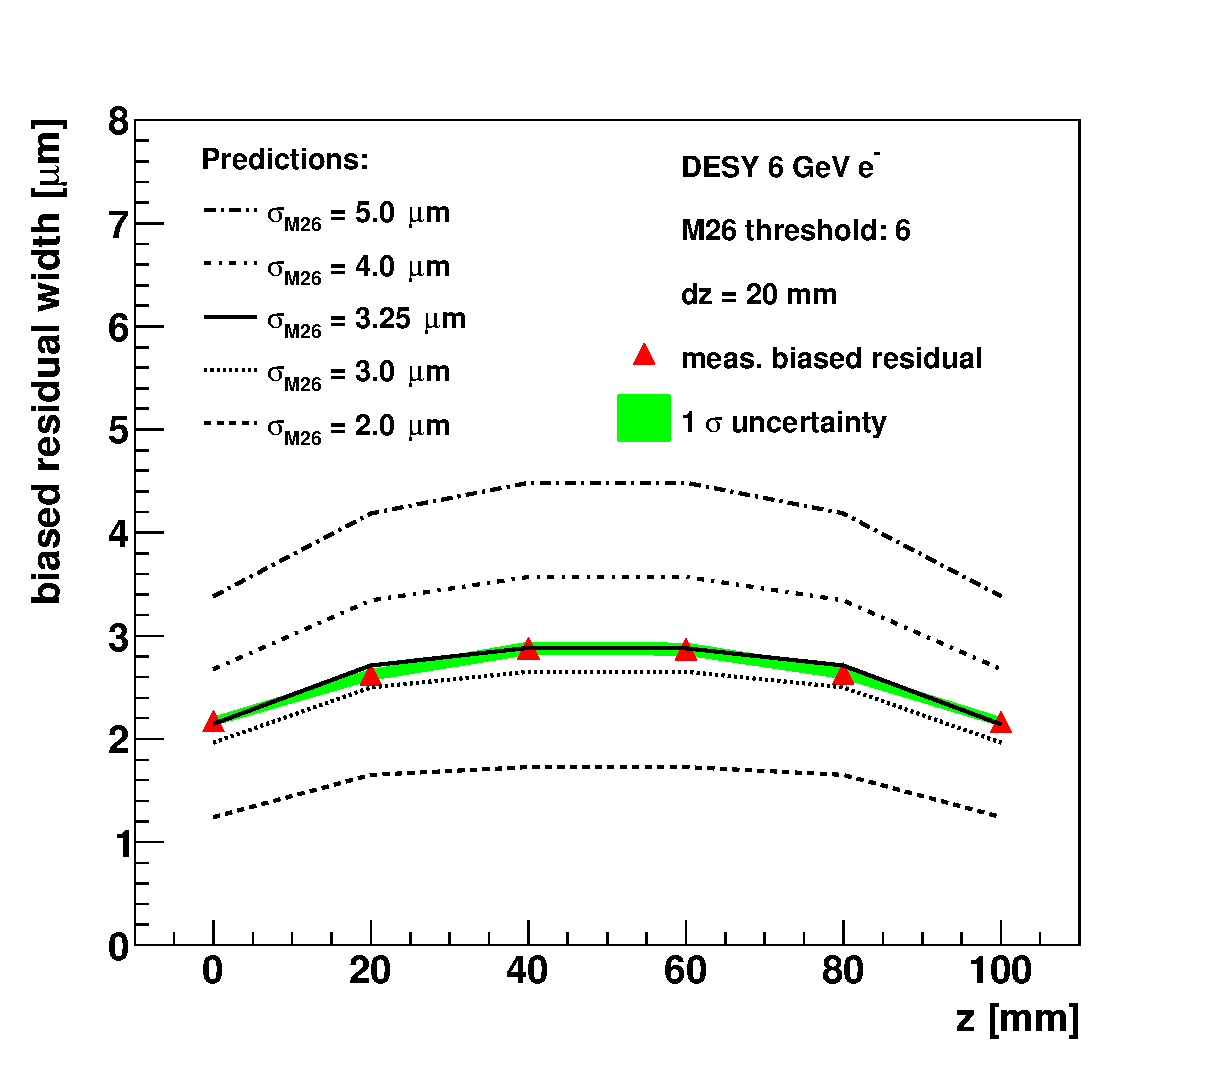
\includegraphics[width=0.49\textwidth]{figures/res_vs_z_20}  \put(-40,146){(A)} % was thin_smiley.pdf
  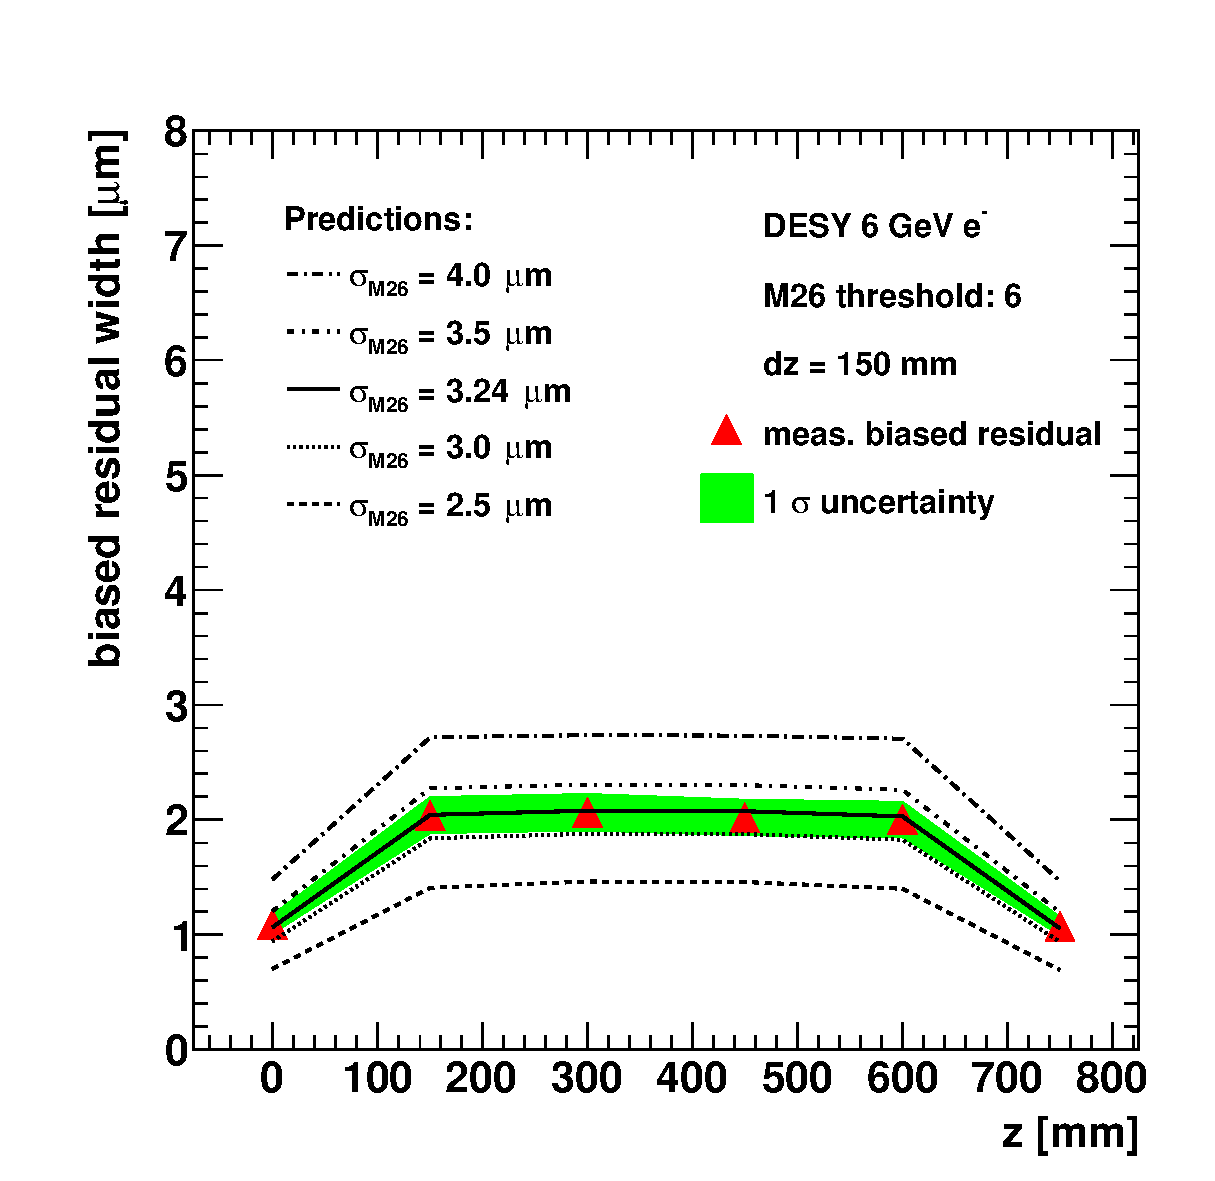
\includegraphics[width=0.49\textwidth]{figures/res_vs_z_150} \put(-40,146){(B)} % was wide_smiley.pdf
  %\caption[Intrinsic telescope sensor resolution at $20\,\milli\meter$ and $150\,\milli\meter$ plane spacing~\cite{ref:thomas}]{Intrinsic telescope sensor resolution at $20\,\milli\meter$ (top)
  % and $150\,\milli\meter$ (bottom) plane spacing.
  \caption[The measured residual widths of each telescope plane.]{
  The measured residual widths of each telescope plane are shown in both the $x$- and $y$-direction for a plane spacing of $\dz = 20\,\milli\meter$ (A) and $\dz = 150\,\milli\meter$ (B).
  The black line shows the predicted residual width at $\sigmam = 3.25\,\upmu\meter$, the green band the measurement standard deviation.
  %Dotted and dashed lines indicate the predicted residual widths, in case differing intrinsic resolutions are assumed.
  %Data was taken at a sensor threshold of $\noise = 6$ and using 6\,GeV electrons at DESY-II.
  %Modified from~\cite{ref:thomas}.
  }
  \label{fig:smiley}
\end{figure}


The six measured residual widths in the $x$-direction for both the narrow plane spacing of $\dz = 20\,\milli\meter$ and the wide spacing of $\dz = 150\,\milli\meter$ are shown in figure~\ref{fig:smiley} (A) and (B)
 at a beam energy of 6\,GeV and a sensor threshold $\noise = 6$, respectively. 
The residuals at a considered plane $i$ are always smaller for the wide configuration in comparison to the narrow one. 
Also, the residuals decrease towards lower beam energies. 
These effects stem from the term $\sigmatb$ in equation~(\ref{eq:telescoperesolutionequation1}): 
(1) Qualitatively, the spatial uncertainty of the extrapolation to the next plane increases with larger lever arms $\dz$. 
(2) The biased track resolution tends towards the intrinsic resolution for increased scattering. 
Hence, the difference between $\sigmai$ and $\sigmatb$ decreases. 

%The energy dependent width of the scattering angle distribution increase the uncertainty with decreasing energy, c.f.\.equation~\ref{eq:multiplescattering}. 
%In the former term, the geometric scaling factor is larger in the wide configuration, in the latter $\sigma_{\textrm{MS}}$ increases with decreasing beam energy. 

%In order to find the best estimate of the intrinsic sensor resolution, a $\chi^2$ minimisation is performed. 
%Inputs to this minimisation are the twelve measured residuals widths $\sigmameas$ at a sensor threshold of $\noise = 6$ and a beam energy of 6\,GeV. 
%These are compared to analytical estimates of the residuals $\sigmahat$, which depend on the known geometry of the set-up, its material budget, the beam energy,
% and the intrinsic sensor resolution, cf.~equation~(\ref{eq:telescoperesolutionequation}). 
%The $\chi^2$ is calculated over all planes as
%
% \begin{equation}
% \label{eq:chi2_sigmai}
% \chi^2 = \sum_{i = 0}^{N-1} \left( \frac{\sigmahat_{i,x} - \sigma_{\textrm{meas},i,x}}{\sigma_{\sigmameas}} \right)^2 + 
% 				    \left( \frac{\sigmahat_{i,y} - \sigma_{\textrm{meas},i,y}}{\sigma_{\sigmameas}} \right)^2,
% \end{equation}

%\noindent
%with the uncertainty of the measured residuals $\sigma_{\sigmameas}$.
%The minimum of equation~(\ref{eq:chi2_sigmai}) with respect to $\sigmai$ is calculated in order to determine the intrinsic sensor resolution $\sigmai$.
%In both cases, an error of $0.5\,\milli\meter$ on the plane distance $\textrm{d}z$ is assumed. % This assumption is done for track fitting. Plane position is fixed in chi2 minimisation for \sigmai

The average intrinsic resolution of the $\Mimosa$ sensors at 6\,GeV and threshold $\noise = 6$ results to
\begin{equation}
 \sigma_{\textrm{M26}} = \left( .\,\pm\, \allowbreak . \right)\,\micro\meter.  
\end{equation}

\noindent
This average is taken over all twelve measured dimensions of the telescope and measurements at plane distances $\dz =  20\,\milli\meter$ and $\dz =  150\,\milli\meter$. 
%The average over the two configurations results in $\sigma_{\textrm{M26}} = \left( 3.43\,\pm\, \allowbreak 0.03 \right)\,\micro\meter$. 
%The stated uncertainty is the error on the mean, the standard deviation is $0.10\,\micro\meter$.
For both geometries, the result is consistent with an earlier analysis that yielded an intrinsic resolution of $\sigmai \approx\,3.5\,\micro\meter$~\cite{ref:mimosa26}.
The following assumptions have been made: 
Firstly, the multiple scattering terms described in equation~(\ref{eq:multiplescattering}) are calculated considering the measured sensor thicknesses, the air between sensor planes, and a $25\,\micro\meter$
thick Kapton foil on either side of each sensor.
%In equation~(\ref{eq:multiplescattering}), the nominal beam energy is used. 
Secondly, the intrinsic resolution $\sigmai$ is assumed to be equal over the area of the sensor. 
%As the discriminator thresholds are set for a total of four subframes per plane individually, this is not necessarily true.
%Figure~\ref{fig:resivsenergy_thresh} shows the dependence of $\sigmai$ on the applied SNR threshold
Additionally, the results are averaged over all cluster sizes. 

%\item Residual widths are calculated using straight line tracks only.
%Inclined tracks, or a deflection of tracks in planes or scattering material, are not taken into account.
%However, as shown in~\cite{ref:lutzpaper}, angular deflections are then considered for the later $\chi^2$ minimisation.

The above method is repeated for different beam energies at a fixed threshold $\noise = 6$. 
This allows for the determination of $\kappa$ as a function of the beam energy. 
The correlation is shown in Figure~\ref{fig:HL_factor}. 
In the energy range covered, $\kappa$ is found to be constant at a value $\kappa = 0.85$ within the uncertainties, which translates to a correction by 15\,\% in comparison to the Highland formula. 

\begin{figure}[ht!]
  \centering
  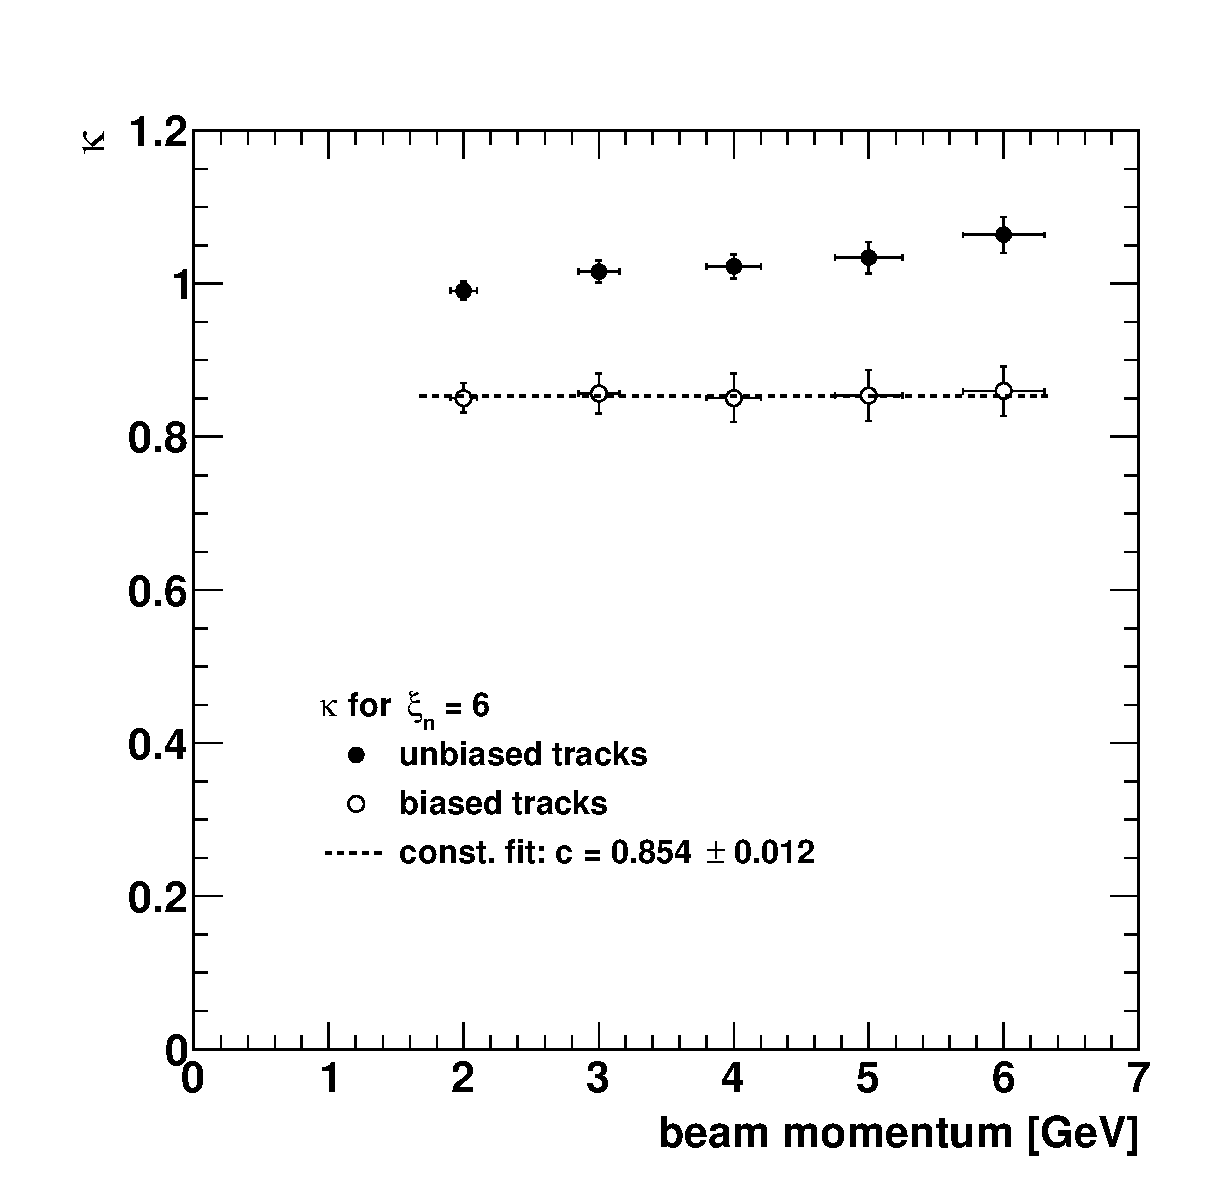
\includegraphics[width=0.49\textwidth]{figures/kappa}
  \caption[HL Factor]{
  The global factor $\kappa$ to the Highland formula is plotted against beam energy.
  }
  \label{fig:HL_factor}
\end{figure}

Furthermore, the method has been repeated for various sensor thresholds.
The threshold applied to each telescope sensor is a critical parameter for the telescope performance.
A higher threshold reduces the amount of fired pixels which results in fewer clusters found on average on a plane and thus limiting the number of reconstructible tracks.
This reduces the sensor efficiency, which is defined as the ratio of reconstructed tracks that have at least one hit on the investigated plane within $d = 100\,\micro\meter$ to the overall number of tracks.
The margin $d$ is additionally scaled with the inverse energy and the plane distance $\dz$. 
In figure~\ref{fig:resivsenergy_thresh}~(A) the efficiency dependence on the sensor threshold is shown for various beam energies and sensor spacings.
Efficiencies are shown exemplary for plane 3. 
Statistical errors are negligible due to the large amount of tracks recorded.
Also, systematic uncertainties are insignificant due to precise alignment and sufficiently large margin $d$.  
For thresholds $\noise < 7$ the efficiency is above $98\,\%$. ??
With increasing threshold, the efficiency decreases until a level of $82\,\%$ at $\noise = 12$ is reached. ??
The efficiency varies by maximal 1\,\% between different set-ups and measurements at a given threshold. 

\begin{figure}[tbp]
  \centering
  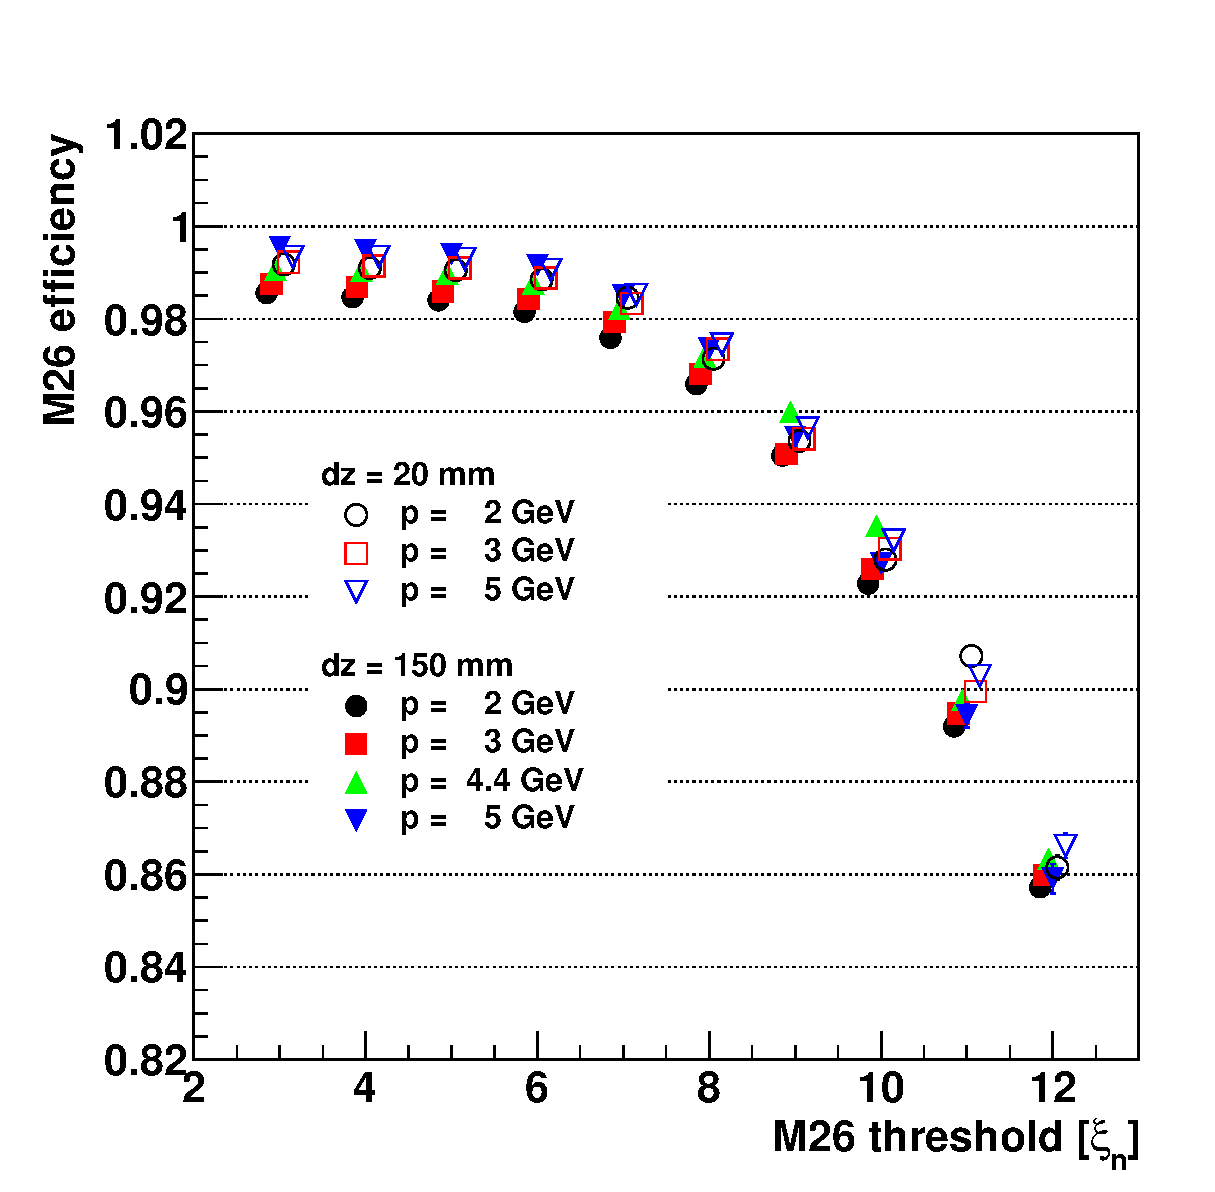
\includegraphics[width=0.49\textwidth]{figures/effi_thresh}		\put(-155,35){(A)}
  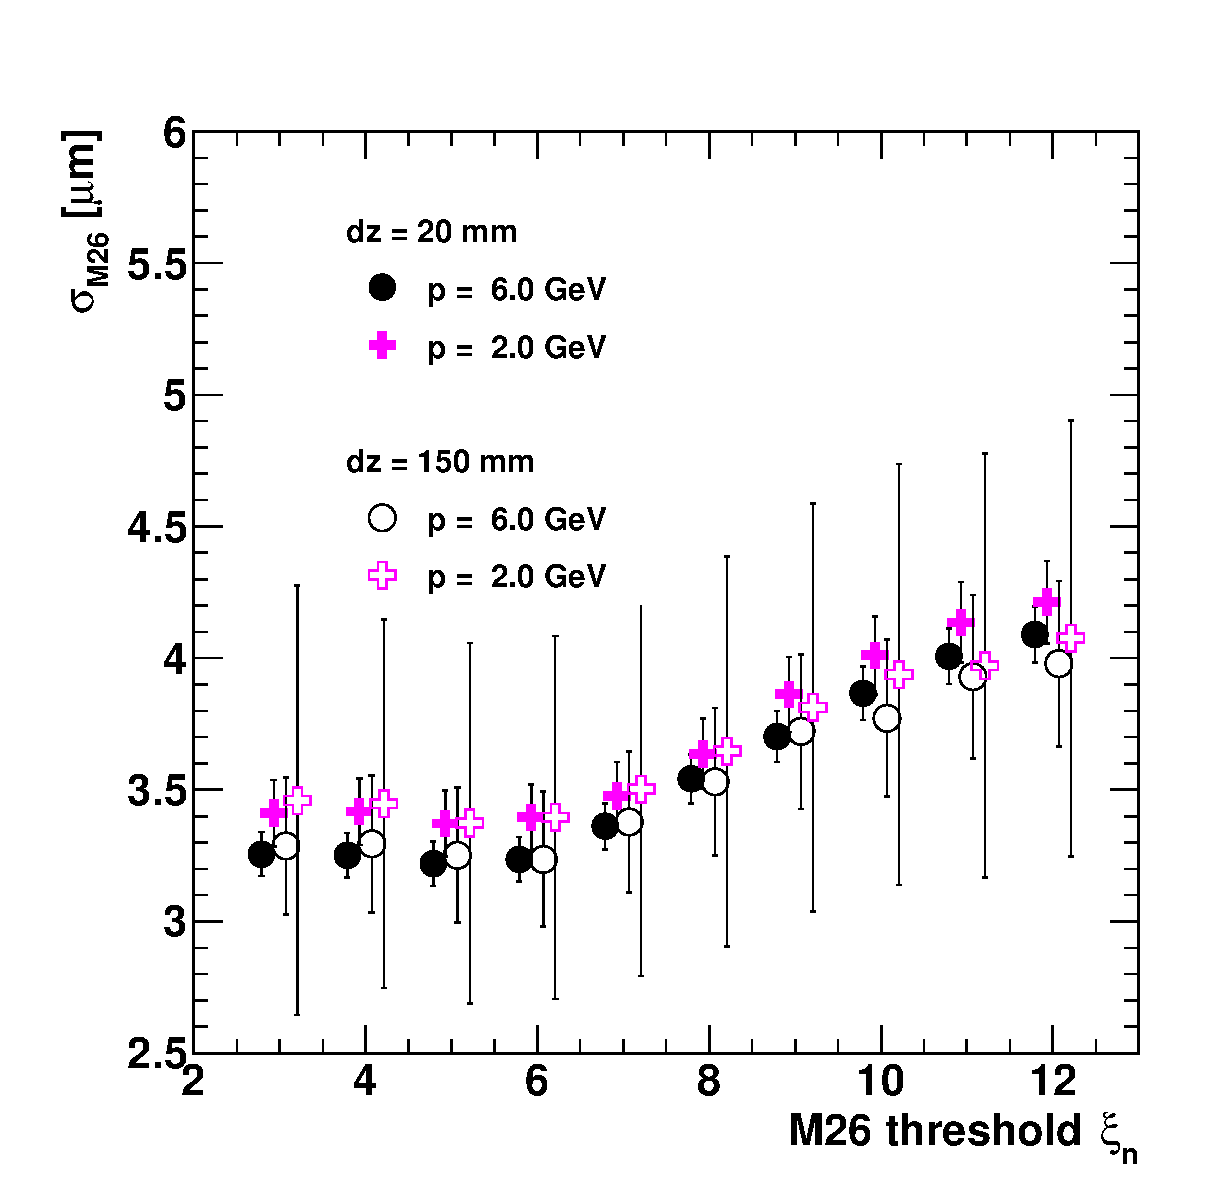
\includegraphics[width=0.49\textwidth]{figures/reso_vs_thres}	\put( -40,35){(B)} % was resi_thresh_errors
  \caption[Telescope intrinsic sensor resolution for different threshold settings, beam energies and geometries~\cite{ref:thomas}]{
(A) Average efficiency of all telescope sensors for different beam energies and sensor spacing vs.~applied threshold.
%An efficiency decline with increasing threshold can be observed.
(B) The measured intrinsic resolution of the $\sigma_{\textrm{M26}}$ for different beam energies $p$ and sensor spacing $\textrm{d}z$ as a function of the applied sensor threshold $\noise$.
In both images values are shifted on the $x$-axis for improved legibility.
Modified from~\cite{ref:thomas}.}
  \label{fig:resivsenergy_thresh}
\end{figure}

The threshold level affects not only the efficiency, but also the intrinsic resolution. 
With an increased threshold, a hit is formed from smaller clusters which deteriorates its position estimate. 
A deterioration also occurs towards lower thresholds allowing for an increased number of noise induced signals to pass the zero-suppression on the chip.
%Figure~\ref{fig:effi} shows the efficiency distribution over a sensor plane.
%As maximum distance $100\,\micro\meter$ is considered.
%A noisy pixel column at $Y \approx -8\,\milli\meter$ can be observed.
%This column was masked during the converter step in the \texttt{datura-noDUT} example and subsequently is not used during the analysis. 
%\\{comment hj: datura-noDUT is jargon}
%Disregarding this area, an overall average efficiency over $98\,\%$ is observed.
%each resulting in an estimate for $\sigmai$ as a function of the set threshold $\noise$. 
Figure~\ref{fig:resivsenergy_thresh} (B) shows the intrinsic sensor resolutions $\sigmai$ derived from the measurements for different beam energies and plane distances as a function of the applied sensor threshold.
The minimum of $\sigmai$ is reached for a sensor threshold setting of $\noise = 5$~to~6.
The difference in intrinsic resolution for different energies and for different plane spacings is less than $.\,\upmu\meter$ ?? for thresholds $\noise > $ ??. 
A previous measurement and analysis by Behr~\cite{ref:j.behrmeasurements} taken at $\noise\,>\,10$ yielded $\sigma_{\textrm{M26}} = (4.35\,\pm\,0.10)\,\micro\meter$, which overestimates the the intrinsic resolution. 



\subsection{Track resolution predictions using General Broken Lines}

%The track resolution of a beam telescope represents the accuracy with which a track can be pointed on a DUT. 
% In case multiple scattering cannot be neglected, it can be expressed as
% \begin{equation}
%  \sigmap^2 = \sigma_{\textrm{Tel}}^2 + \sigma_{\textrm{MS}}^2
% \end{equation}
% 
% \noindent
Using the measured intrinsic resolution, the known material budget $\epsmimo = 7.6\cdot 10^{-4}$ of the sensor planes including the Kapton protection and the material budget of a DUT $\epsdut$,
 predictions of the expected track resolution at the actual DUT position $\zdut$, c.f.\ figure~\ref{fig:datura_sketch}, can be made.
Therefore, it is possible to perform an a priori calculation of the optimal telescope geometry for a certain measurement set-up. 
In this section, $\zdut$ is assumed to be in the centre between plane\,2 and plane\,3.

%Track resolutions in this section refer to the achievable track resolution using a \textit{symmetric six M26 planes plus DUT} configuration. 
%This is referred to as \textit{user configuration}, also shown in figure~\ref{fig:datura_sketch}, while the set-up used in section~\ref{sec:measurements} is referred to as \textit{gauge configuration}. 

Using the GBL formalism, the track resolution is analytically calculated at points of interest along the particle trajectory. 
The track resolution at the DUT for four different DUT material budgets $\epsdut$ is depicted as a function of the spacing $\dzdut$ in figure~\ref{fig:CalcResos_dzdut}.
Exemplified are two configurations with $\dz = 20\,\milli\meter$ and $\dz = 150\,\milli\meter$ at (A) DESY-II and (B) SPS beam energies. 
For $\dz = \dzdut = 20\,\milli\meter$ at 5\,GeV beam energy the track resolution at the DUT is 
\begin{equation}
 \sigmatb(\zdut) = 1.9\,\upmu\meter
\end{equation}

\noindent
for $\epsdut = 0.001$.
This analytical prediction has no uncertainty. 
%The uncertainty originates from an assumed uncertainties of 5\,\% on the beam energy and 10\,\% on the material budget. 
For SPS energies, a track resolution of $1.4\,\upmu\meter$ is predicted. ??
The shown resolution functions monotonically increase with increasing $\dzdut$. 
In order to achieve the best possible resolution, the inner $\Mimosa$ planes should, therefore, be positioned as close as possible to the DUT, i.e.~$\dzdut$ is to be minimised. 
In addition, figure~\ref{fig:CalcResos_dzdut} shows, that the optimal plane spacing $\dz$ depends on the actual DUT size along the beam direction and its material budget.
For instance for a DUT with a material budget of $\epsdut = 0.001$ (solid lines) at 5\,GeV, a narrow configuration shows a higher resolution for $\dzdut < 70\,\milli\meter$,
 while a wide configuration is best for $\dzdut > 70\,\milli\meter$.
The intersection is marked with an arrow in figure~\ref{fig:CalcResos_dzdut}. 
The position of the intersection of the two lines depends on the material budget of the DUT $\epsdut$ and shifts to smaller $\dzdut$ with increasing material budget. 
%A DUT with a material budget of $\eps$
%In the wide (narrow) configuration, the predicted track resolution on the DUT is about $2.4\,\upmu\meter$ ($1.9\,\upmu\meter$) at $\dzdut = 20\,\milli\meter$ for DUTs with $\epsdut = 0.001$.
At SPS energies, the resolution functions for the wide and the narrow configuration do not intersect, with the narrow configuration showing a slightly better
However, the difference is less than $0.5\,\micro\meter$ for $\zdut = 100\,\milli\meter$ even for $\epsdut = 0.03$. 

\begin{figure}[tbp]
  \centering
  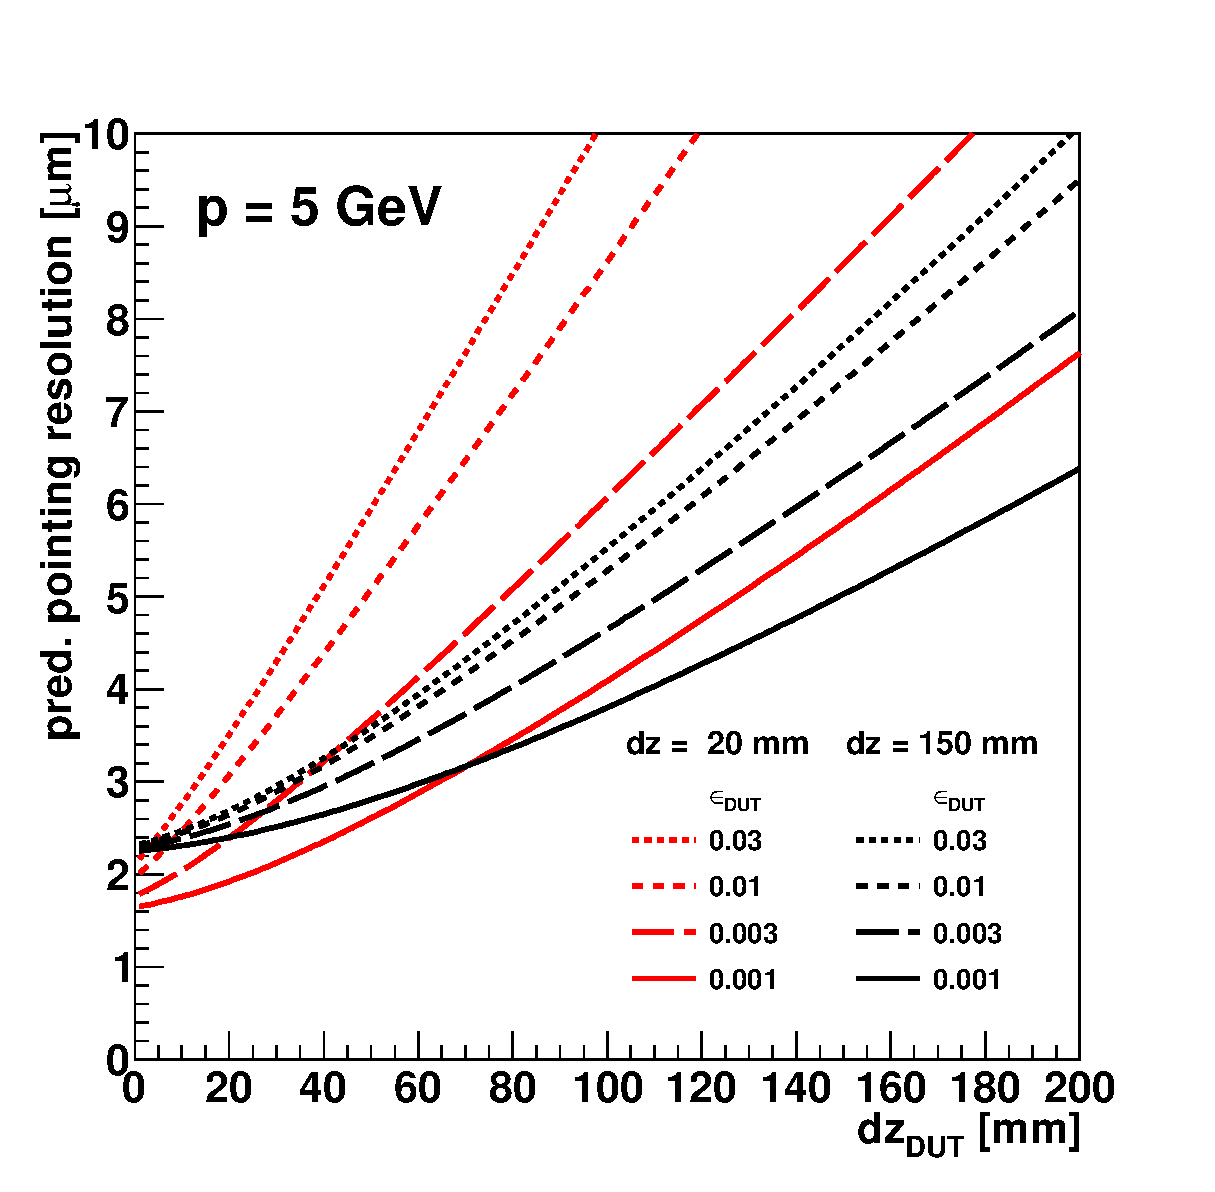
\includegraphics[width=0.49\textwidth]{figures/CalcResoVsDzdut_Desy2}\put(-165,35){(A)}\put(-128,58){$\uparrow$}
  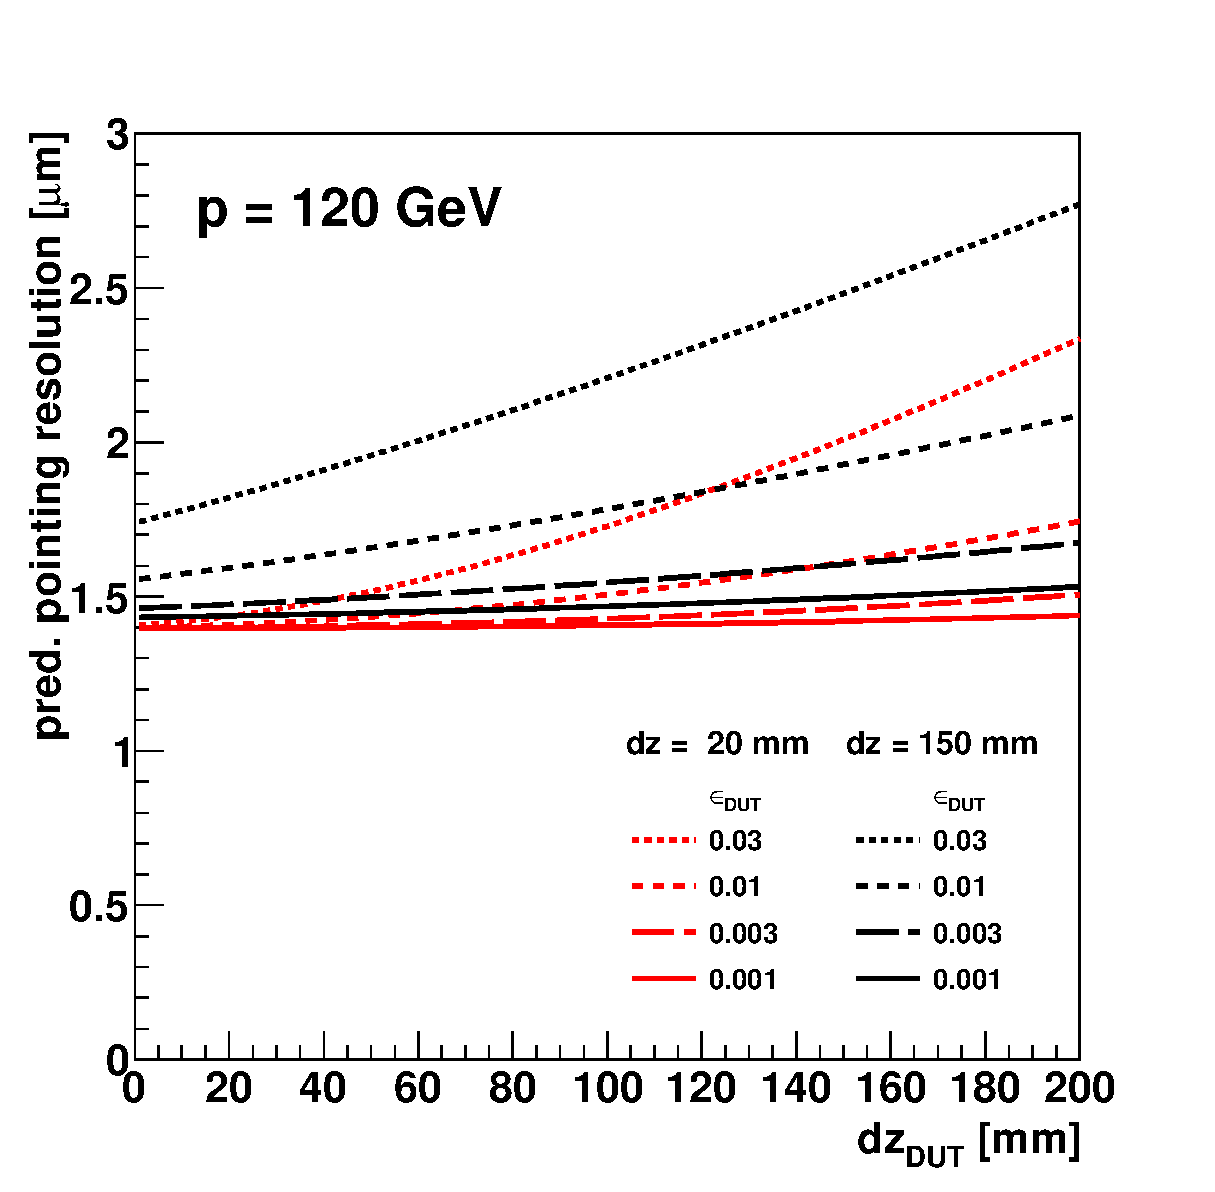
\includegraphics[width=0.49\textwidth]{figures/CalcResoVsDzdut_Cern2}\put(-165,35){(B)}
  %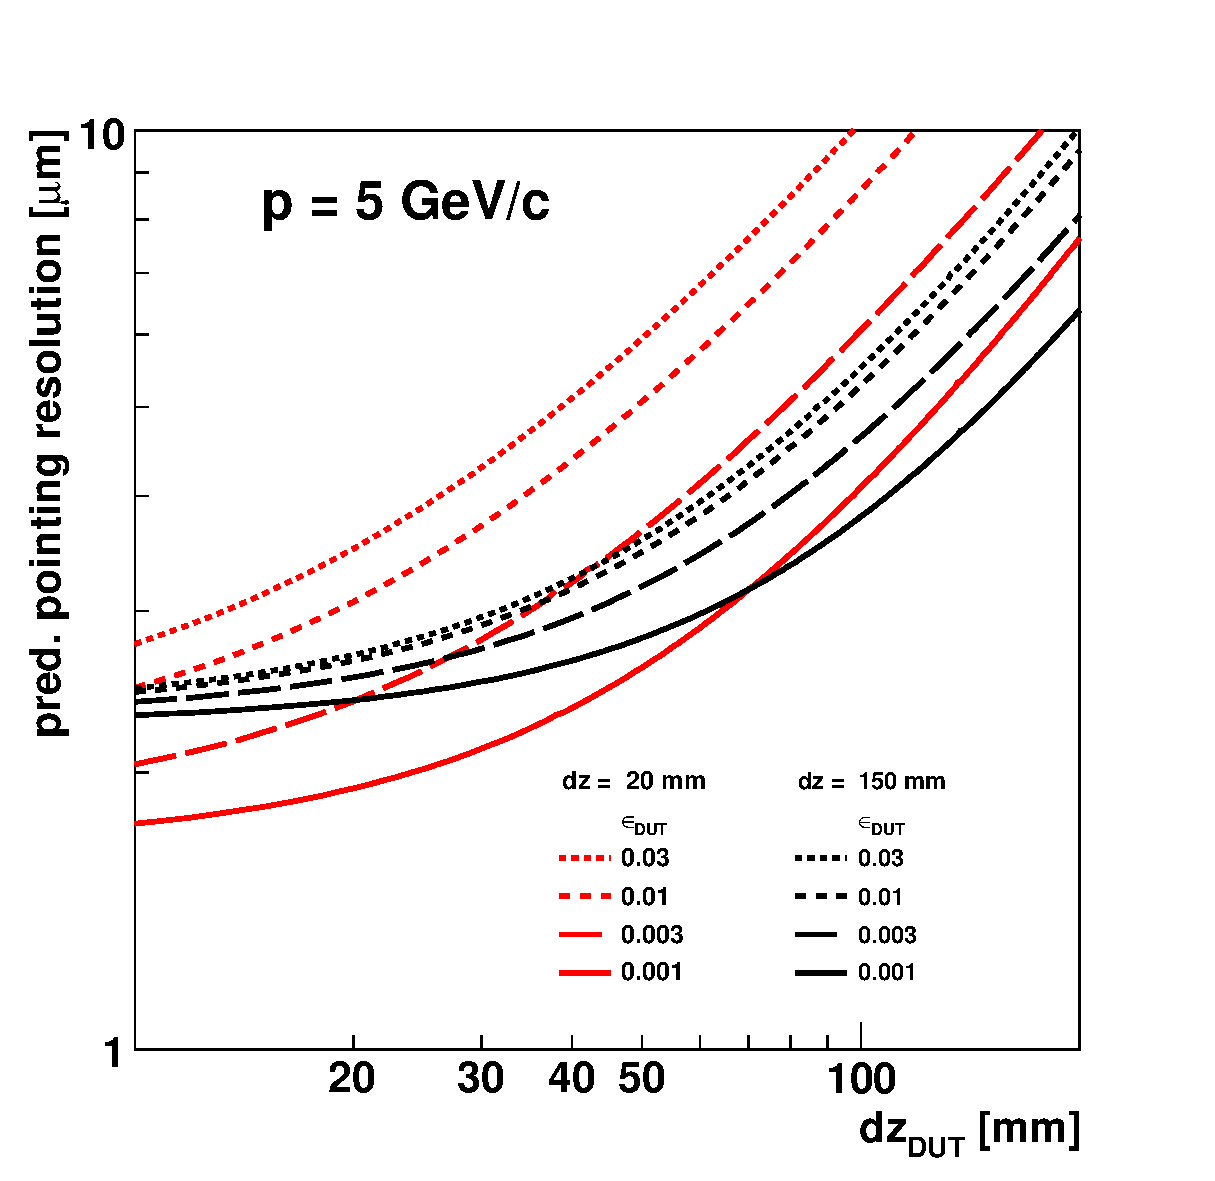
\includegraphics[width=0.49\textwidth]{figures/CalcResoVsDzdut_Desy_loglog_2}
  %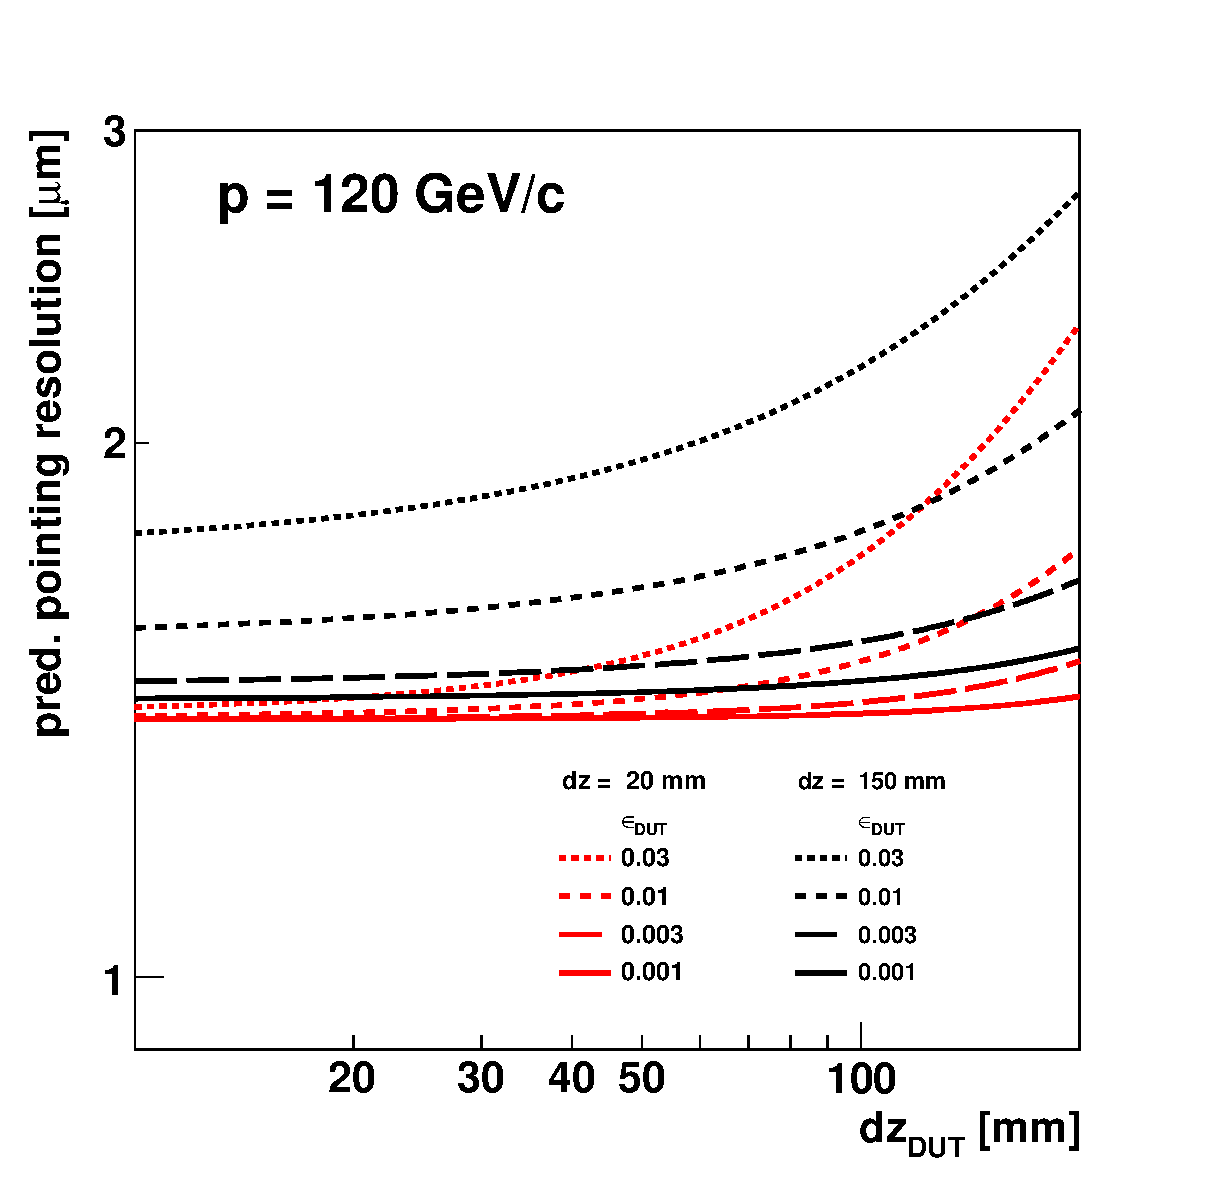
\includegraphics[width=0.49\textwidth]{figures/CalcResoVsDzdut_Cern_loglog_2}
  \caption[Track resolution for various material budgets as a function of the distance between DUT and neighbouring planes]{
  The track resolution for various material budgets is shown as a function of the equidistant spacing between DUT and neighbouring planes at 5\,GeV (A), and 120\,GeV (B)
  at the centre of the beam telescope ($\zdut$).}
  \label{fig:CalcResos_dzdut}
\end{figure}

% Using the \textit{gauge configuration}, a comparison between the GBL calculations and the measurements can be performed.
% For this, the measured resolution has to be converted to the track resolution $\sigmap$ by correcting for the intrinsic resolution of the DUT $\sigmadut = \sigmam$
% 
% \begin{equation}
%  \sigmap = \sqrt{\sigmameas^2 - \sigmadut^2}.
%  \label{eq:sigmap}
% \end{equation}
% 
% \noindent
% This is shown in figure~\ref{fig:CalcResoP_DUT} (A) as a function of the beam energy. 
% The solid lines represent GBL calculations, while the triangles show the derived $\sigmap$ obtained from equation~(\ref{eq:sigmap}). 
% The hatched bands represent the calculated track resolution assuming $\sigmam = 3.43\,\upmu\meter$ with a standard deviation of $0.10\,\upmu\meter$ for the wide and the narrow configuration. 
% An excellent agreement between GBL calculations and the measurements is found. 
% For the limit towards high energies, or negligible multiple scattering, a track resolution of $1.6\,\upmu\meter$ is predicted. 
% The measurement at 120\,GeV confirms the prediction, 

In figure~\ref{fig:CalcResoP_DUT} the achievable track resolution at $\zdut$ as a function of the material budget is shown at 5\,GeV.
%Again, a minimal $\dzdut$ allows for the best possible resolution. 
Dashed and solid lines represent calculations for $\dz = 20\,\milli\meter$ and $\dz = 150\,\milli\meter$, respectively. 
The track resolution deteriorates with increasing $\epsdut$. 
The optimal plane spacing $\dz$ depends on the actual size requirements for the DUT along the beam direction and its material budget.
For instance, for a DUT with a material budget of $\epsdut = 0.002$, a plane spacing of $\dz = 20\,\milli\meter$ should be used, if $\dzdut$ is as small as 20\,mm. 
However, a plane spacing of $\dz = 150\,\milli\meter$ is preferred, if $\dzdut$ is 60\,mm or larger. 
Intersections are marked with open circles. 
For $\epsdut$ below (above) the intersection, a narrow (wide) configuration is preferable. 
The position of the intersection shifts to smaller material budgets with increasing $\dzdut$. 

\begin{figure}[tbp]
  \centering
  %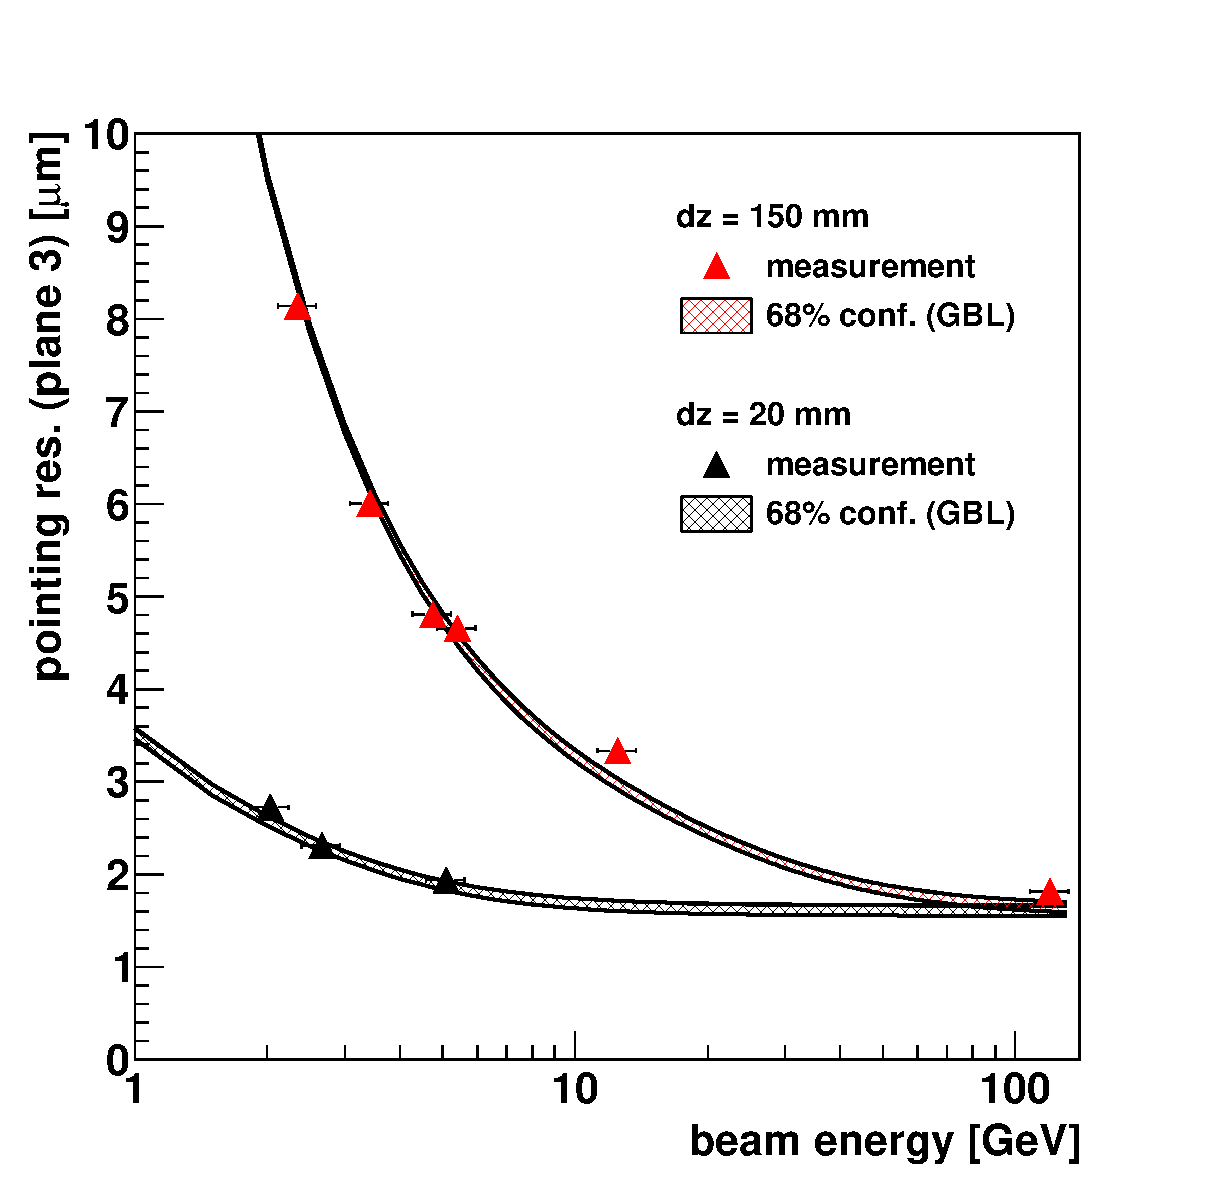
\includegraphics[width=0.49\textwidth]{figures/energy_plot}     \put(-175,40){(A)} % was CalcResoVsP
  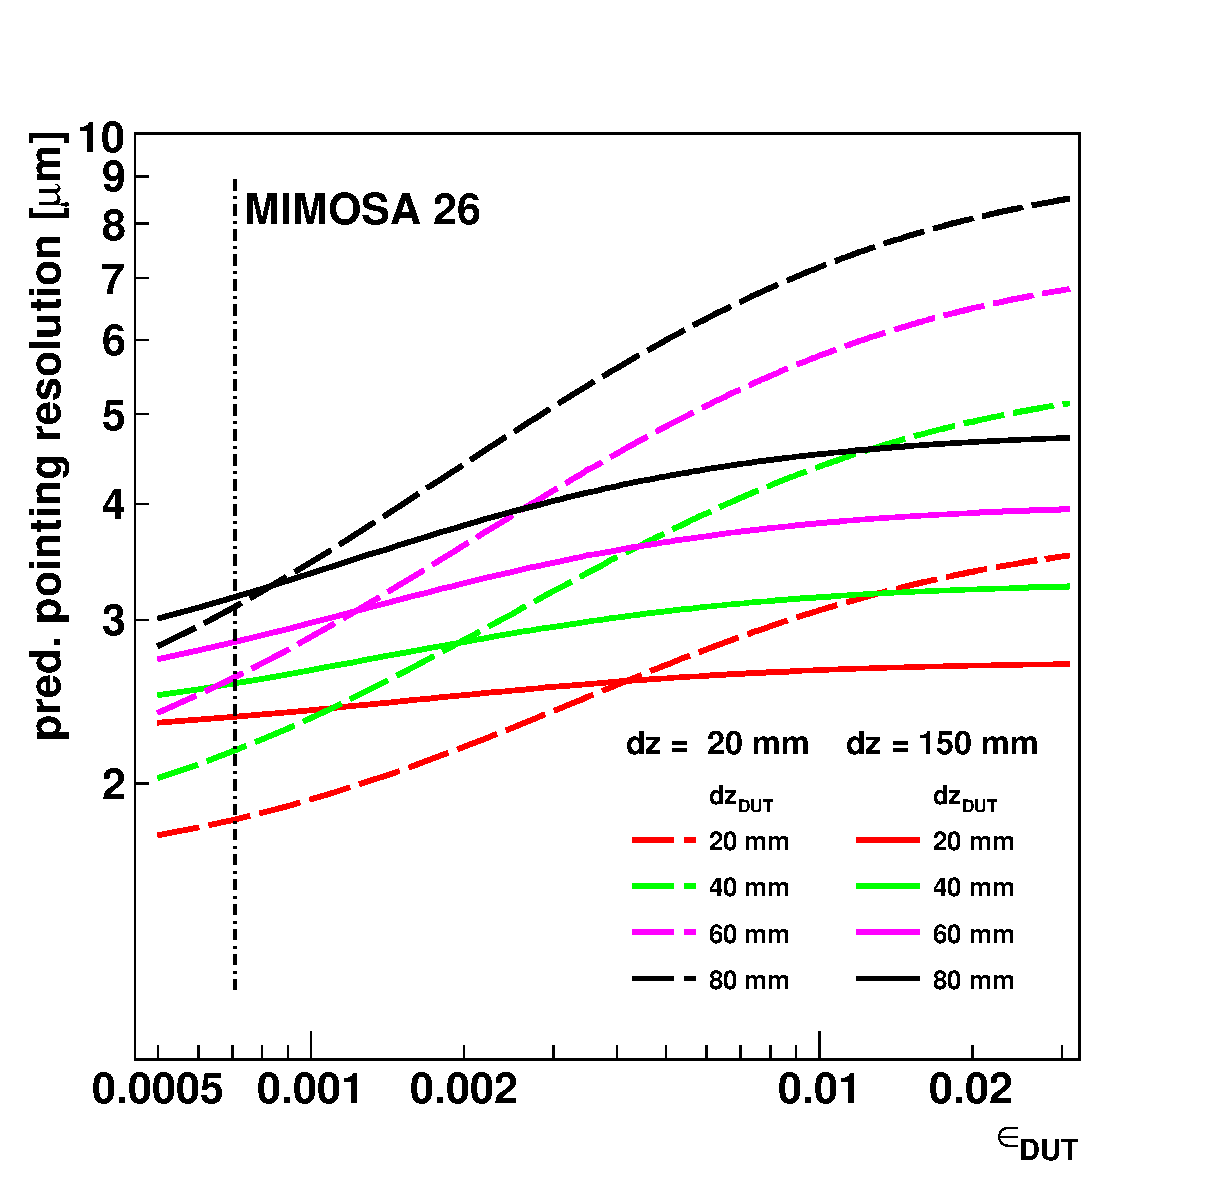
\includegraphics[width=0.49\textwidth]{figures/CalcResoVsEpsdut} %\put(-155,40){(B)}
%               \put(-175,107.5){$\bigcirc$}
%  \color{blue} \put(-161,102.5){$\bigcirc$}
%  \color{green}\put(-143,96.5){$\bigcirc$}
%  \color{red}  \put(-113,90){$\bigcirc$}
%  \color{black}
   \caption[Track resolution as a function of the beam energy]{
   %(A) The measured (triangles) and calculated (lines) track resolution at plane $3$
   % for the wide (red) and the narrow (black) set-up is shown as a function of the beam energy for the \textit{gauge configuration}~\cite{ref:thomas}. 
   %The solid lines form bands representing the standard deviation of $0.10\,\upmu\meter$ of the intrinsic resolution.
   %The theoretical limit of about $1.6\,\upmu\meter$ for plane\,3 is indicated as a dashed line.
   %Track resolutions derived from the measured resolutions at plane 3 for various energies and plane spacings are shown as crosses.
   The calculated track resolutions at the DUT for two geometries are shown as a function of $\epsdut$ at $\zdut$ at a beam energy of 5\,GeV. 
   Note the double logarithmic scales. 
   }
 \label{fig:CalcResoP_DUT}
\end{figure}




\section{Considerations for DUT integrations}
\label{sec:dutintegration}
%mechanic
A DUT can be mechanically integrated into the $\DESY$-type beam telescopes at two positions: behind the last telescope plane, or between the two telescope arms.
If placed between the arms, micrometer precision $xy\phi$-stages are available for translation scans and rotation of the DUT~\cite{Mimosa-twiki}.
At this position, the maximum DUT width is 500\,mm.
DUTs with larger spatial dimensions are therefore placed at the rear end of the beam telescope. 

%trigger and daq sw
User DAQ systems are integrated to the TLU the same way as the beam telescope DAQ itself using either the RJ45 or the LEMO interface, cf.~section~\ref{sec:tdaq}.
The handshake mode is configurable for each integrated systems individually. 
For the integration of the DUT data stream with EUDAQ, a producer capable of receiving commands by the Run Control and sending data to the $\eudaq$ Data Collector is necessary,
 as described in section~\ref{sec:eudaq}.

%eutelescope
A dedicated alignment run prior to the installation of the DUT allows for precise alignment of the telescope planes, especially for larger $\epsdut$. 
With a proper alignment at hand, runs including a DUT are to be analysed subsequently in order to align the DUT with respect to the beam telescope. 
The reconstructed tracks can then be used to characterise the DUT, i.e.~to measure its intrinsic resolution or its detection efficiency. 

With increasing $\epsdut$, and thus multiple scattering within the DUT, the choice of the tracking processor needs further consideration. 
In general, a GBL fit produces tracks with a lower $\chi^2$ compared to straight line fits,
 as kinks at the possibly thick DUT and also at the $\Mimosa$ planes themselves are not allowed for in the straight line fit.
Therefore, using GBL for track fitting is recommended. 
% The inclusion of downstream planes using straight line fits might significantly deteriorate the resolution,
If straight line fitting is used nevertheless, a fit using only the upstream planes might result in a narrower unbiased residual width, compared to a fit that includes the downstream planes. 
This is due to a bias of the extrapolated tracks at the DUT by the downstream planes after traversing material. 
For comparison, in a narrow \textit{user configuration} using a 6\,GeV electron/positron beam, the pointing resolution of the $\DESY$-type beam telescope at the DUT using GBL is $1.83\,\upmu\meter$. 
The optimal configuration using only the upstream planes is a wide configuration with $\dz = 150\,\milli\meter$,
 and the achievable pointing resolution is above $3.88\,\upmu\meter$. 
Hence, using only the upstream planes deteriorates the resolution by more than $2\,\upmu\meter$.

A web tool yielding compatible results in comparison with the GBL calculations is available~\cite{webtool}.

\section{Conclusion}
\label{sec:conclusion}

%Test beam measurements with high precision pixel beam telescopes have proven to be a versatile tool for a wide range of semiconductor sensor studies. 
%Among other beam telescopes, also the DESY-type beam telescopes are used as a key ingredient for many sensors R\&D projects. 

The highly flexible and versatile DESY-type beam telescopes come with a complete data acquisition system, a Trigger Logic Unit with time stamping capabilities
 and a clearly defined interface for an integration of user data acquisition systems.
It also provides the powerful software packages $\eudaq$, a modular data acquisition framework, and $\EUTelescope$ for data analysis. 
% to intro X users used a DESY-type beam telescopes only in 2013 for a total of n weeks alone at the DESY-II test beam areas. 
This work the performance of the  DESY-type beam telescopes has been investigated. 
At 5\,GeV beam energy, a measured unbiased residual width of $(3.96 \pm 0.03)\,\upmu\meter$ is achievable
 and the intrinsic resolution of the $\Mimosa$ sensors have been measured to $(3.43 \pm 0.03)\,\upmu\meter$.
General Broken Lines calculations predict a pointing resolution of $1.89\,\upmu\meter$ on the DUT in a \textit{five planes plus DUT} configuration with 20\,mm plane spacing,
 which well agrees wit a measured pointing resolution of $(1.94 \pm 0.08)\,\upmu\meter$.

A continuous development is ongoing to upgrade and enhance the data acquisition system itself, and also the data acquisition and analysis framework.  
The maximum achievable rate will be increased by the successor of the TLU, allowing for a trigger rate of up to 1\,MHz.
%This is only possible with the implementation of parallel data streams for the telescope planes and the DUT, which will be available with \eudaq\,{2.0},
% which will incorporate a new event format supporting multiple triggers per $\Mimosa$ read-out frame. 
 A new data format will support multiple triggers per mimosa read-out frame facilitating asynchronous data acquisition. 
The development of the $\EUTelescope$ analysis software is driven by the large and diverse user community. 
Features currently under development include tracking in magnetic fields and more accurate detector geometry descriptions. 

Future versions of \eudaq\ will provide support for asynchronous data streams allowing to operate certain devices at a much higher trigger frequency than others
 and thus making full use of the the beams available in the various beam lines.




\section*{Acknowledgements}
We, the authors, are indebted to Claus Kleinwort for his counsel and numerous discussions. 
Also, we would like to thank Ulrich K\"otz and Jan Dreyling-Eschweiler. 
The test beam support at DESY is highly appreciated. 
This work was supported by the Commission of the European Communities under the FP7 Structuring the European Research Area, contract number RII3-026126 (EUDET). 
Furthermore, strong support from the Helmholtz Association and the BMBF is acknowledged.
%contract number RII3-CT-2006-026126.
%Funding agencies AIDA, EUDET

\small
\bibliographystyle{IEEEtran}
\bibliography{bibtex/refs}

\end{document}


